% =====================================================================
%  FloodLite: A CPU-and-Browser Edge-Deployment Benchmark for
%             Lightweight Flood Segmentation
%  Authors: Tasfia Noor Chowdhury, Md Ibrahim Khalil (corresponding)
%  Target venue: Elsevier International Journal of Disaster Risk Reduction (IJDRR),
%                double-blind. Build the author-free manuscript file with
%                   latexmk -pdf main_blind.tex   (defines \BLIND, see below)
%                and the author-bearing version with  latexmk -pdf main.tex.
%  Previous venue: Environmental Modelling & Software, ENVSOFT-D-26-03981, desk-rejected 2026-11-09.
%  Numbers source of truth:
%       code/runs/3fold/{summary,quantized,lat_m2,lat_wasm}.json
%       code/runs/3fold/{ptq_mechanism,ptq_mobilevit_groups}.json  (T12, S5.3)
%       code/runs/host2/*.json                                      (T13, S5.4)
%       code/runs/3fold/zero_shot_3fold.json                        (T9, S5.8)
%       code/runs/combined/{quantized,quantized_pc}.json            (T11, S5.9)
%  Tables source of truth: docs/tables.md
%  Status: v2 draft (post edge-benchmark pivot, 2026-05-16).
% =====================================================================

% Submission layout: single column, double spaced, with line numbers
% (elsarticle [preprint,review]).  For a two-column camera-ready preview,
% use [final,3p,times,twocolumn] and remove \linenumbers below.
\documentclass[preprint,review,12pt]{elsarticle}
\usepackage{lineno}
\usepackage[margin=1in]{geometry}  % wider text block so wide tables stay legible
\usepackage{adjustbox}            % shrink-to-fit for wide tables (tables/*.tex)

% ---------- Packages ----------
\usepackage[T1]{fontenc}
\usepackage[utf8]{inputenc}
\usepackage[british]{babel}
\usepackage{graphicx}
\usepackage{amsmath,amssymb}
\usepackage{booktabs}
\usepackage{array}
\usepackage{url}
\usepackage{xcolor}
\usepackage[hidelinks]{hyperref}
\usepackage{textcomp}
\usepackage{tabularx}
\usepackage{caption}
\usepackage{multirow}
\usepackage{siunitx}
\sisetup{detect-weight=true,detect-family=true}
\usepackage{microtype}            % subtle character protrusion + font expansion

% ---------- Macros for FloodLite numbers ----------
% Headline numbers; update here and they propagate through the text.
\newcommand{\teacherIoU}{0.9257}
\newcommand{\teacherStd}{0.0078}
\newcommand{\bestStudentIoU}{0.9367}
\newcommand{\bestStudentStd}{0.0055}
\newcommand{\bestStudent}{MobileViT-XXS}
\newcommand{\deployableModel}{EfficientNet-Lite0}
\newcommand{\deployableINTIoU}{0.8851}
\newcommand{\deployableINTStd}{0.0149}
\newcommand{\deployableINTDelta}{-0.0426}
\newcommand{\deployableMTwoFPS}{58}
\newcommand{\deployableWASMFPS}{6}
\newcommand{\teacherMTwoFPS}{26.6}  % teacher ORT-CPU FPS (ORT 1.17); PyTorch-eager was 3.6

% ---------- Double-blind switch ----------
% \BLIND is defined by main_blind.tex. In the blind build the author block,
% CRediT, acknowledgements, funding and competing-interest sections are
% omitted (they go in the separate title page), and the repository URLs
% that name the authors' accounts are masked.
\ifdefined\BLIND
  \newcommand{\repoURL}{[code-repository URL withheld for double-blind review]}
  \newcommand{\combinedURL}{[dataset URL withheld for double-blind review]}
\else
  \newcommand{\repoURL}{\url{https://github.com/NoorTasfia/flood-segmentation}}
  \newcommand{\combinedURL}{\url{https://www.kaggle.com/datasets/tasfianoorchowdhury/flood-combined-fsegnet}}
\fi

% Convenience commands.
\newcommand{\Cn}{C\textsubscript{n}}
\newcommand{\ie}{i.e.,\ }
\newcommand{\eg}{e.g.,\ }

% ---------- Front matter ----------
\journal{International Journal of Disaster Risk Reduction}

\begin{document}
\linenumbers

% Allow TeX to break lines more loosely; tight column justification
% with long \texttt{} paths otherwise produces huge inter-word gaps.
\sloppy

\begin{frontmatter}

\title{FloodLite: A CPU-and-Browser Edge-Deployment Benchmark for Lightweight Flood Segmentation}

\ifdefined\BLIND\else
\author[rme]{Tasfia Noor Chowdhury\corref{cor1}}
\ead{tasfiaa.chowdhury@gmail.com}
\author[iit]{Md Ibrahim Khalil\corref{cor1}}
\ead{mik858692@gmail.com}

\affiliation[rme]{
  organization={Department of Robotics and Mechatronics Engineering, University of Dhaka},
  city={Dhaka},
  postcode={1000},
  country={Bangladesh}
}
\affiliation[iit]{
  organization={Institute of Information Technology, University of Dhaka},
  city={Dhaka},
  postcode={1000},
  country={Bangladesh}
}

\cortext[cor1]{Corresponding authors.}
\fi

% --- Abstract + keywords ---
% =====================================================================
%  Section 0 -- Abstract
%  Grounded in code/runs/3fold/*.json and code/runs/combined/*.json;
%  no placeholders. IJDRR limit: 250 words (checked with the plain-text
%  count in scratch/plain_abstract.py; macros expand to numbers).
% =====================================================================

\begin{abstract}
Flood-segmentation models are judged by accuracy, yet responders run them on laptops and browsers, where latency, quantization and false alarms decide whether a model is usable. \emph{FloodLite} benchmarks three compact UNets (MobileNetV3-Small, EfficientNet-Lite0 and MobileViT-XXS encoders) against a larger UNet$+$EfficientNet-B0 reference network on the Flood Semantic Segmentation Dataset (FSSD), measuring FP32 and INT8 latency on two CPUs and in browser WebAssembly, and ablating knowledge distillation (KD). On this saturated benchmark the pretrained compact networks match or exceed the reference network without distillation (IoU $\bestStudentIoU$ vs.\ $\teacherIoU$), and no KD configuration helps. Under the default per-tensor INT8 post-training quantization recipe, EfficientNet-Lite0 loses 0.043 IoU while MobileNetV3-Small, MobileViT-XXS and the reference network lose 0.22--0.52. Per-channel weight scales repair every convolutional network (MobileNetV3-Small $-0.023$, reference network $-0.009$), also after retraining and under zero-shot transfer; MobileViT-XXS keeps a 0.26 loss in its early convolutions. EfficientNet-Lite0 INT8 runs at \deployableMTwoFPS~FPS on an Apple M2~Pro, $2.2\times$ faster and about $4\times$ smaller than the reference network, but $2.8\times$ slower than FP32 on an x86 desktop. Because FSSD contains no water-free images, every FSSD-trained model predicts water on 70--100\% of dry scenes. Retraining on a combined corpus with 855 water-free images cuts false-alarm rates to 3--9\%; there, distillation raises flood IoU by 0.03--0.07 but also copies the reference network's false alarms, 2.3--2.6 times as often. For unattended monitoring, water-free training data is a requirement, and a network must be audited for false alarms before it is distilled from. Code, checkpoints and ONNX exports are released.
\end{abstract}


\begin{keyword}
flood segmentation \sep edge computing \sep knowledge distillation \sep post-training quantization \sep lightweight neural networks \sep ONNX Runtime \sep false alarms
\end{keyword}

\end{frontmatter}

% --- Body sections ---
% =====================================================================
%  Section 1 -- Introduction
% =====================================================================

\section{Introduction}
\label{sec:intro}

Floods are the most frequent and economically damaging natural disasters globally, accounting for 38.7\% of natural disasters and affecting 43\% of disaster-affected populations between 2000 and 2009~\cite{du2010health}. Rapid urbanisation continues to amplify exposure~\cite{hemmati2020urban}. Because traditional hydrological and hydraulic models suffer from high computational demand, coarse spatial resolution, and limited real-time adaptability~\cite{kumar2023flood}, deep-learning segmentation has emerged as a leading approach to automated flood-extent delineation from satellite, drone, and ground imagery~\cite{bentivoglio2022deep}.

Recent benchmark studies in this space have converged on encoder--decoder architectures (UNet~\cite{ronneberger2015unet}, SegNet~\cite{badrinarayanan2017segnet}, and DeepLabV3$+$~\cite{chen2018encoder}) paired with strong feature-extraction backbones, most commonly EfficientNet~\cite{tan2019efficientnet} and ResNet~\cite{he2016deep}. Karc{\i} \emph{et al.}~\cite{karci2026deep} provide the most comprehensive systematic comparison of these combinations on the public Flood Semantic Segmentation Dataset (FSSD), reporting that UNet $+$ EfficientNet achieves the highest segmentation performance (IoU 0.927, F1 0.957, accuracy 0.971) and conclude that this combination ``is ideal for near real-time operational deployment.''

A careful reading of the broader flood-segmentation literature, however, reveals that this operational-deployment claim has not actually been evaluated. Across the 26 related works surveyed by Karc{\i} \emph{et al.}~\cite{karci2026deep} and adjacent studies on SAR~\cite{pechmay2023flooded} and multi-modal flood mapping~\cite{chamatidis2024vision}, nearly every paper reports segmentation accuracy alone. The exception, Hern\'andez \emph{et al.}~\cite{hernandez2022flood}, times PSPNet/DeepLabV3$+$/U-Net on the GPUs and ARM CPUs of NVIDIA Jetson boards, where the largest configurations fail to run on the Jetson Nano at all. But, to our knowledge, \emph{no study reports laptop-CPU or in-browser latency for RGB flood segmentation together with post-quantization accuracy and quantization stability.} This omission is consequential. UNet $+$ EfficientNet-B7, the configuration favoured in~\cite{karci2026deep}, has approximately 63\,M parameters and 50\,GFLOPs at $256{\times}256$ input resolution. Such a model is impractical on the drones, embedded sensors, Raspberry-Pi-class community stations, or offline tablet apps of the kind used in field response to flood zones, where reliable internet connectivity is the exception rather than the rule~\cite{munawar2021review}.

These properties matter for disaster risk reduction because each maps onto a decision. The Sendai Framework calls for preparedness for effective response and for wider access to early warning and disaster-risk information~\cite{unisdr2015sendai}. A flood-segmentation model contributes to either only if it runs where the responder is, on hardware already there and without a network link (latency and size); if a compressed version can be trusted as much as the original (quantization stability); and, when it watches a site unattended as part of a warning chain, if it stays quiet when there is no flood (false-alarm rate on water-free scenes). Segmentation accuracy on a flood-only benchmark answers none of these questions.

\subsection{Contributions}
\label{sec:contributions}

This paper makes four contributions.

\begin{enumerate}
\item \textbf{A CPU-and-browser edge-deployment benchmark for flood segmentation.} We report FP32 and INT8 inference latency for three lightweight UNet students and the teacher on two commodity CPUs (an Apple M2~Pro and an AMD Ryzen~5 desktop, both via ONNX Runtime CPU) and in browser WebAssembly SIMD (ONNX Runtime Web 1.17 and 1.22), together with per-model parameter counts, FLOPs at $256{\times}256$, ONNX disk size, and FP32-to-INT8 size-reduction factors. ONNX is the deployment hub: every measured latency reflects the same exported artifact running under a different execution provider. The two CPUs disagree on the sign of the INT8 speedup: the same INT8 artifact runs $1.3$--$2.0\times$ faster than FP32 on the M2~Pro and $2.8$--$3.0\times$ slower on the Ryzen, so INT8 deployment decisions have to be made per CPU. Measurement on physically constrained edge devices (Raspberry~Pi, mobile SoCs, embedded ARM) is out of scope for this study and deferred to future work (Section~\ref{sec:limitations}). Prior and concurrent edge-oriented flood-segmentation work targets CUDA-equipped Jetson boards~\cite{hernandez2022flood,schmalstieg2026distillation}; we characterise the GPU-free deployment envelope that field laptops, tablets, and web browsers actually provide.

\item \textbf{When knowledge distillation helps flood segmentation, and what it transmits.} On FSSD, across three architectures $\times$ four KD configurations $\times$ three folds, no KD configuration improves on the no-KD baseline: ImageNet-pretrained lightweight students match or exceed the UNet$+$EfficientNet-B0 teacher without distillation. A per-image paired bootstrap over the pooled held-out set ($n=399$ images) confirms this; after Holm correction, response-only and combined KD are significantly \emph{harmful} for MobileViT-XXS. We attribute the result to the saturated 663-image benchmark leaving the teacher no headroom. On a less saturated combined corpus, where the teacher does out-segment the students, combined KD raises flood-only IoU significantly for all three students. It also passes on the teacher's false alarms on water-free scenes. Distillation transfers the teacher's errors along with its skill, so the teacher has to be audited for the deployment-relevant failure first.

\item \textbf{Where INT8 post-training quantization fails, and why.} Under the default ONNX static QDQ INT8 recipe (Percentile 99.999\% calibration, per-tensor scales for weights and activations, Conv/Gemm/MatMul quantized), EfficientNet-Lite0 quantizes cleanly ($\Delta \mathrm{IoU} = -0.043 \pm 0.016$) while MobileNetV3-Small and MobileViT-XXS collapse by 0.45--0.52 IoU with fold-dependent outcomes (cross-fold standard deviations of 0.19--0.34), the teacher loses 0.19--0.30, and the same split reappears after retraining on a second corpus. A controlled ablation that changes one recipe setting at a time (Section~\ref{sec:results-quant}) shows that for every convolutional network this is a recipe artefact, not an architecture property: per-channel weight scales alone bring MobileNetV3-Small to $-0.023 \pm 0.006$ IoU and the teacher to $-0.009 \pm 0.004$, recover MobileNetV3-Small after retraining and under zero-shot transfer as well, and keeping its HardSwish layers in FP32 adds nothing, although their activation range is $12$--$17\times$ wider than ReLU6's. MobileViT-XXS is the exception: it loses 0.22--0.33 IoU under every full-quantization recipe we tried on FSSD and collapses outright after retraining, and a layer-group diagnostic places the loss in its two early high-resolution convolutional stages, not in the attention blocks the transformer-quantization literature would blame~\cite{lin2022fqvit}. The implication for practitioners: \emph{switch on per-channel weights before concluding that a backbone cannot be quantized; MobileViT-XXS is the one backbone here for which that is not enough.}

\item \textbf{The false-alarm failure of flood-only training data, and its remedy.} Beyond the cross-sensor Sen1Floods11 collapse (Section~\ref{sec:results-ood}), we evaluate every FSSD-trained model, FP32 and INT8, on two \emph{within-regime} RGB test sets whose disjointness from FSSD we verify by perceptual-hash deduplication: AIFloodSense (94 ground-level images) and the held-out FloodNet test split (424 UAV images, 215 water-free). FP32 students transfer as well as the teacher (0.69--0.72 IoU), but every FP32 model false-alarms on 70--100\% of water-free scenes, a consequence of flood-only training data that no FSSD-internal metric reveals. INT8 degradation also grows under domain shift, up to outright collapse of the architectures that already quantized marginally in-domain. Retraining on a combined corpus that includes water-free images brings student false-alarm rates down to 3--9\% and flood-only IoU on FloodNet up to 0.70--0.78, which turns the failure into a concrete data requirement for unattended flood monitoring.
\end{enumerate}

We make our trained checkpoints, the ONNX FP32 and INT8 exports, the per-platform benchmarking harnesses, and the full code repository publicly available; a tagged release of the submitted version will be archived on Zenodo with a persistent DOI upon acceptance.

\subsection{Scope and pivot from initial framing}
\label{sec:scope-pivot}

This work was originally framed as a knowledge-distillation recipe for compressing a heavy flood-segmentation teacher. The empirical results did not support that framing, and we report the negative-KD finding rather than search for a configuration that would justify the original framing. The contribution pivots to the per-platform edge benchmark, the diagnosis of INT8 post-training quantization failures, and the conditions under which distillation pays off. Testing the negative result on a second, less saturated corpus showed that it is a property of the benchmark rather than of distillation, and that where distillation does help it carries a cost the headline IoU does not show. We hope this is more useful to practitioners than another KD recipe.

The remainder of the paper is organised as follows. Section~\ref{sec:related} reviews relevant prior work on flood segmentation, lightweight segmentation backbones, knowledge distillation, and post-training quantization. Section~\ref{sec:methods} details the FloodLite methodology. Section~\ref{sec:experimental-setup} describes the experimental setup, including the 3-fold protocol and per-platform latency rigging. Section~\ref{sec:results} reports results across Tables~\ref{tab:t1-footprints}--\ref{tab:t13-host2} and Figures~\ref{fig:f2-pareto}--\ref{fig:f4-throughput}. Section~\ref{sec:discussion} discusses the negative-KD finding, per-platform deployment recommendations, and the PTQ diagnosis. Section~\ref{sec:limitations} lists limitations. Section~\ref{sec:conclusion} concludes.

% =====================================================================
%  Section 2 -- Related Work
% =====================================================================

\section{Related work}
\label{sec:related}

\subsection{Deep learning for flood segmentation}
\label{sec:rw-flood}

Convolutional encoder--decoder architectures dominate the deep-learning flood-segmentation literature. Pech-May \emph{et al.}~\cite{pechmay2023flooded} applied U-Net to Sentinel-1 SAR imagery for flooded-area detection. Bahrami and Arbabkhah~\cite{bahrami2024enhanced} compared SegNet, UNet, and FCN32 for floodplain segmentation, reporting SegNet's max-pooling indices as advantageous on smooth water-surface transitions. Patil \emph{et al.}~\cite{patil2024flood} used an ensemble of ResNet34, InceptionV3, and VGG16 on Sentinel-1 SAR for flood-damage assessment, reaching an IoU of 0.758. Ghosh \emph{et al.}~\cite{ghosh2024automatic} used a Nested U-Net with FPN and EfficientNet-B7 backbone on the NASA IEEE GRSS benchmark, reporting that models trained on specific events generalise to new geographies. Chamatidis \emph{et al.}~\cite{chamatidis2024vision} introduced Vision Transformers (ViT) to the task and reported a 9--15\% improvement over comparable CNN baselines on Sentinel-1 and Sentinel-2 imagery. Most recently, Karc{\i} \emph{et al.}~\cite{karci2026deep} performed the most comprehensive systematic comparison to date, evaluating UNet, SegNet, and DeepLabV3$+$ each with EfficientNet and ResNet backbones, and concluded that UNet $+$ EfficientNet is the strongest configuration on FSSD.

Across this body of work, model efficiency is almost entirely absent from the evaluation. Hern\'andez \emph{et al.}~\cite{hernandez2022flood} are the notable exception: they benchmark PSPNet, DeepLabV3$+$, and U-Net inference times for UAV flood detection on three CUDA-equipped NVIDIA Jetson boards (Nano, TX2, AGX Xavier), on both GPU and CPU. Their study, however, targets GPU-accelerated edge devices, retains heavy backbones (DeepLabV3$+$ cannot run on the Nano with any encoder, and UNet$+$EfficientNet runs only on the Xavier, at $\sim$14\,s per image on CPU), and does not consider quantization. Outside the UAV setting, Mateo-Garcia \emph{et al.}~\cite{mateogarcia2021onboard} demonstrated flood segmentation running on the hardware accelerator of a CubeSat-class satellite (PhiSat-1) so that only flood masks need downlinking. This is the clearest demonstration to date that flood models must sometimes run \emph{where the data is}, albeit on multispectral imagery and bespoke onboard hardware. Concurrently with this work, Nie \emph{et al.}~\cite{nie2026gated} demonstrated real-time CPU-only SAR flood segmentation on satellite internet terminals, and Bhattacharjya \emph{et al.}~\cite{bhattacharjya2026floodreasonbench} benchmarked vision--language reasoning segmentation for flood response on a Jetson AGX Xavier, which shows that deployability is becoming a first-class concern in this literature. To the best of our knowledge, however, no prior or concurrent flood-segmentation study measures inference latency on commodity CPUs (Apple Silicon class) or in a browser WebAssembly sandbox, and none quantifies the per-architecture stability of INT8 post-training quantization for this task.

\subsection{Knowledge distillation for semantic segmentation}
\label{sec:rw-kd}

Knowledge distillation (KD), introduced by Hinton \emph{et al.}~\cite{hinton2015distilling} and surveyed comprehensively by Gou \emph{et al.}~\cite{gou2021kdsurvey}, trains a small student network to match the soft outputs of a larger teacher. Romero \emph{et al.}~\cite{romero2015fitnets} extended this to feature-space alignment with FitNets, training the student to match intermediate feature representations through a learned adapter. For dense-prediction tasks, Liu \emph{et al.}~\cite{liu2019structured} proposed structured-knowledge distillation (SKD) that aligns pairwise pixel similarities; Wang \emph{et al.}~\cite{wang2020intra} proposed inter- and intra-class distance distillation specifically for segmentation; and He \emph{et al.}~\cite{he2021channel} introduced channel-wise KD for compact segmentation models. These methods routinely achieve compression ratios of $5$--$20\times$ with sub-1\% mIoU degradation on Cityscapes and ADE20K. Concurrently with this work, Schmalstieg \emph{et al.}~\cite{schmalstieg2026distillation} distilled a 300M-parameter geospatial foundation model (Prithvi-EO-2.0) into a 0.7M-parameter EfficientViT student for Sentinel flood mapping, deploying it as a quantization-aware-trained INT8 TensorRT engine on a Jetson Xavier NX. Their setting differs from ours in modality (satellite multispectral imagery vs.\ heterogeneous ground/aerial RGB), distillation goal (multiplying a fixed annotation budget with teacher-generated labels vs.\ transferring response and feature knowledge to an already-strong student), and quantization route (QAT on an edge GPU vs.\ PTQ on CPU). To our knowledge, no prior work ablates classical response- and feature-based KD for flood segmentation.

Two findings from the broader KD literature are particularly relevant here. First, KD gains shrink sharply as student capacity and pretraining quality grow, and a stronger teacher is frequently \emph{not} a better teacher~\cite{romero2015fitnets,cho2019efficacy,beyer2022patient}. Second, distillation can succeed at its own objective while failing to improve the student: Stanton \emph{et al.}~\cite{stanton2021does} show that student--teacher fidelity and student generalisation routinely diverge, so on saturated benchmarks where the student matches or exceeds the teacher without distillation, the response-based term reduces to a noise-injection regulariser rather than a genuine transfer signal. Our empirical results on FSSD (Section~\ref{sec:results-kd}) are consistent with both observations.

\subsection{Lightweight backbones for mobile vision}
\label{sec:rw-backbones}

MobileNetV3~\cite{howard2019searching} uses neural architecture search and the H-swish activation to produce CPU-friendly classification networks; the Small variant has approximately 2.5\,M parameters. EfficientNet-Lite~\cite{tan2019efficientnet} is a quantization-friendly redesign of EfficientNet that removes squeeze-and-excitation and Swish activations to ease INT8 conversion, with the Lite0 variant containing approximately 4.7\,M parameters. MobileViT~\cite{mehta2022mobilevit} introduces hybrid CNN--Transformer blocks; the XXS variant has only 1.3\,M parameters yet is competitive with much larger models on ImageNet. MobileNetV2~\cite{sandler2018mobilenetv2}, included as an off-the-shelf baseline in this work, predates these but remains a strong reference point and exhibits the ReLU6-bounded activation profile we associate with PTQ stability (Section~\ref{sec:results-quant}). We adapt all four as encoders in a U-Net-style decoder.\footnote{The parameter counts quoted here are \emph{backbone-only} (encoder) figures from the classification literature. The full segmentation models we train and deploy add a shared U-Net decoder; their complete encoder$+$decoder parameter counts, which are the deployment-relevant figures, are reported in Table~\ref{tab:t1-footprints} (e.g.\ MobileViT-XXS is 1.3\,M as a backbone but 3.09\,M as a full UNet).}

Beyond the four classification-derived backbones we evaluate, several segmentation-specific lightweight architectures have been proposed. BiSeNetV2~\cite{yu2021bisenetv2} uses a two-pathway design (spatial $+$ context) optimised for real-time urban-scene segmentation. PIDNet~\cite{xu2023pidnet} reframes the three-pathway split as a proportional--integral--derivative controller. Fast-SCNN~\cite{poudel2019fastscnn} targets sub-150-MB-FLOP inference at $1024{\times}2048$. We do not evaluate these in this work because (a)~they are designed for and benchmarked on Cityscapes-style urban scenes, not the heterogeneous viewpoints (aerial / oblique / ground) of FSSD, and (b)~our objective is to characterise the deployability of the \emph{commodity} UNet $+$ ImageNet-pretrained-backbone family that the flood-segmentation literature has already converged on, not to propose a new architecture.

\subsection{Post-training quantization}
\label{sec:rw-ptq}

Post-training quantization (PTQ) maps FP32 weights and activations to lower-precision integer representations~\cite{jacob2018quantization,krishnamoorthi2018quantizing,gholami2021quantsurvey}. Two main flavours exist: dynamic PTQ, which only quantizes weights and computes activation ranges at inference time, and static PTQ, which calibrates activation ranges offline against a representative dataset. For convolutional networks, the ONNX static QDQ (Quantize--DeQuantize) format with per-channel weight quantization and per-tensor activation quantization is the \emph{de facto} standard~\cite{ortQuant} and is supported across major edge runtimes (ONNX Runtime CPU, TensorFlow Lite, CoreML). The conventional wisdom that ``INT8 PTQ retains accuracy within 1 IoU point of FP32''~\cite{krishnamoorthi2018quantizing} is derived from classification networks with bounded-range activations (ReLU, ReLU6) on ImageNet-scale benchmarks. The same literature warns that depthwise-separable networks need per-channel weight scales: Krishnamoorthi~\cite{krishnamoorthi2018quantizing} reports MobileNet-family models falling to near-zero accuracy under per-tensor weights. As we show in Section~\ref{sec:results-quant}, this warning carries over to flood segmentation, where the default per-tensor recipe collapses three of our four networks and per-channel scales recover every convolutional one. The transformer-quantization literature attributes PTQ failure in attention blocks to severe inter-channel variation at LayerNorm inputs and non-uniform attention distributions~\cite{lin2022fqvit,li2023repqvit}; for MobileViT-XXS we find the attention blocks quantize cleanly and the loss sits in the convolutional trunk instead. Edge-deployment field studies report that quantized MobileNetV3 can silently collapse to constant outputs depending on kernel and calibration choices~\cite{qiu2022mlexray}, which matches the fold-dependent collapse we observe under per-tensor weights.

\subsection{On-device disaster response}
\label{sec:rw-ondevice}

Operational disaster-response platforms must function under intermittent connectivity, limited power, and heterogeneous hardware. Edge AI in humanitarian contexts has been explored by Munawar \emph{et al.}~\cite{munawar2021review} and Kuglitsch \emph{et al.}~\cite{kuglitsch2022facilitating}. The operational state of the art, UNOSAT's CNN-based rapid-mapping service~\cite{nemni2020rapid}, cuts flood-map production time by $\sim$80\% but runs server-side on downlinked Sentinel-1 imagery, so it presumes connectivity that post-disaster field teams often lack. At the opposite end of the hardware spectrum, the TinyML community has standardised latency/energy benchmarking for sub-watt devices~\cite{banbury2021mlperftiny} and demonstrated ImageNet-scale inference on microcontrollers~\cite{lin2020mcunet}, while in-browser inference is an established deployment channel for JavaScript runtimes~\cite{smilkov2019tfjs}. The deployment platforms we benchmark, Apple Silicon CPU and browser WebAssembly, sit between these poles and correspond to two real operational profiles: field-laptop and UAV inference, and citizen-science web portals. Raspberry-Pi-class single-board computers, AWS Graviton ARM CPU, and Android edge targets are discussed in Section~\ref{sec:limitations} as straightforward but unscheduled extensions.

% =====================================================================
%  Section 3 -- Materials and Methods
% =====================================================================

\section{Materials and methods}
\label{sec:methods}

\begin{figure*}[t]
\centering
\includegraphics[width=0.95\linewidth]{figures/F1_pipeline.pdf}
\caption{\textbf{FloodLite training-and-deployment pipeline.} Train teacher (UNet$+$EfficientNet-B0) $\rightarrow$ train students (three lightweight backbones $\times$ four KD configurations) $\rightarrow$ INT8-quantize the no-KD students via ONNX static QDQ $\rightarrow$ benchmark FP32 and INT8 on Apple M2~Pro CPU and in browser WebAssembly. Each stage produces an artifact consumed by the next; the same \texttt{.onnx} file is benchmarked under two execution providers (ONNX Runtime CPU on M2~Pro; ONNX Runtime Web WASM SIMD in the browser).}
\label{fig:f1-pipeline}
\end{figure*}

Figure~\ref{fig:f1-pipeline} summarises the four-stage workflow. The remainder of this section details each stage.

\subsection{Datasets}
\label{sec:methods-data}

\paragraph{FSSD.} We use the public Flood Semantic Segmentation Dataset (FSSD)~\cite{fssd2024kaggle}, which is also the evaluation dataset of Karc{\i} \emph{et al.}~\cite{karci2026deep} and therefore enables direct head-to-head comparison. FSSD comprises 663 RGB images of flood-affected areas, each at $512{\times}512$\,px, paired with binary segmentation masks (flood $=1$, non-flood $=0$). Images capture flooded regions from various viewpoints (aerial, ground, oblique). We resize all images and masks to $256{\times}256$\,px and normalise pixel values to $[0,1]$ followed by ImageNet mean/std normalisation.

We partition the pooled data with a fixed random seed, \texttt{KFold(n\_splits=5, shuffle=True, random\_state=42)}, and evaluate three folds $\{0,1,2\}$ of this five-fold partition (each held-out fold is 20\% of the data; we refer to this as three-fold evaluation, not three-fold cross-validation). We disclose that the reduction from five to three folds was made \emph{after} fold~0 had shown no benefit from distillation, to save compute; it is therefore a data-dependent design decision. The three folds were fixed by index before any of folds~1--2 were run, every model and KD configuration uses the same folds, and the powered per-image bootstrap of Section~\ref{sec:setup-stats} pools all 399 held-out images of these folds. We report all results as mean $\pm$ standard deviation across the three folds, and explicitly caveat all paired-Wilcoxon p-values for low statistical power (minimum reportable two-sided p-value at $n=3$ is 0.25).

Each training run keeps the checkpoint of the epoch with the highest IoU on its held-out fold, and Tables~\ref{tab:t2-segmentation}--\ref{tab:t5-latency} report that same fold, so the in-distribution numbers carry a small optimistic selection bias that is shared by every configuration and therefore cancels in the paired contrasts. The external test sets of Sections~\ref{sec:results-ood}--\ref{sec:results-combined} are never used for checkpoint selection or any other decision and are free of it.

\paragraph{External zero-shot test sets.} For the within-regime generalization evaluation (Section~\ref{sec:results-zeroshot}) we use two held-out subsets of a combined public flood corpus: the official FloodNet v1.0 test split~\cite{rahnemoonfar2021floodnet} (424 UAV images, 215 of them water-free; CDLA-Permissive), with the \emph{water} and \emph{road-flooded} classes mapped to flood, and the AIFloodSense test split~\cite{simantiris2026aifloodsense} (94 ground-level images; CC~BY~4.0). Neither set is used for training or model selection anywhere in this paper. A perceptual-hash duplicate check between all 663 FSSD images and all 3{,}009 images of the combined corpus (DCT pHash, Hamming distance $\leq 8$) found \emph{zero} near-duplicate pairs, so these evaluations are free of train--test leakage by construction; the check is reproducible via \texttt{scripts/check\_fssd\_overlap.py} and its report ships with the code release. The corpus additionally fixes duplicate-aware training folds over the CC0-licensed Kaggle Flood Area Segmentation images~\cite{karim2022floodarea} and FloodNet train$+$val, which we use for the negative-image-bearing retraining experiment of Section~\ref{sec:results-combined} (its loader, manifest-driven splits, and source-balanced sampler are part of the released code).

\subsection{Reference network (teacher)}
\label{sec:methods-teacher}

The larger reference network, which plays the teacher in the distillation experiments and is referred to as the teacher below, is a UNet decoder with EfficientNet-B0 encoder~\cite{tan2019efficientnet}, initialised from ImageNet weights. While Karc{\i} \emph{et al.}~\cite{karci2026deep} use EfficientNet-B7 in their best-performing configuration, we deliberately choose B0 as our teacher for two reasons: first, B0 is significantly cheaper to train, fitting within free-tier GPU budgets (Kaggle T4 and Google Colab); second, B0 is itself representative of the strongest configurations realistically used in practice, and with only 663 training images a larger backbone is unlikely to provide additional headroom (Section~\ref{sec:results-teacher}). The teacher has approximately 6.25\,M parameters at $256{\times}256$ resolution.

\subsection{Compact networks (students) and the MobileNetV2 baseline}
\label{sec:methods-students}

We evaluate three compact UNet configurations, the students in distillation terms, together with a MobileNetV2~\cite{sandler2018mobilenetv2} off-the-shelf baseline of the teacher's size class, which tests whether the teacher's EfficientNet-B0 encoder confers any advantage over a generic lightweight encoder. Each student replaces the teacher's EfficientNet-B0 encoder with a smaller backbone while keeping the UNet decoder topology identical. All four configurations are initialised from ImageNet weights via the \texttt{segmentation\_models\_pytorch} library~\cite{iakubovskii2019smp} and \texttt{timm}~\cite{wightman2019timm}.

Model footprints (parameter counts and FP32/INT8 ONNX disk sizes) appear in Table~\ref{tab:t1-footprints}.

Figure~\ref{fig:f6-architecture} shows the architecture shared by every model and the points at which the distillation signals of Section~\ref{sec:methods-kd} attach.

\begin{figure*}[ht]
\centering
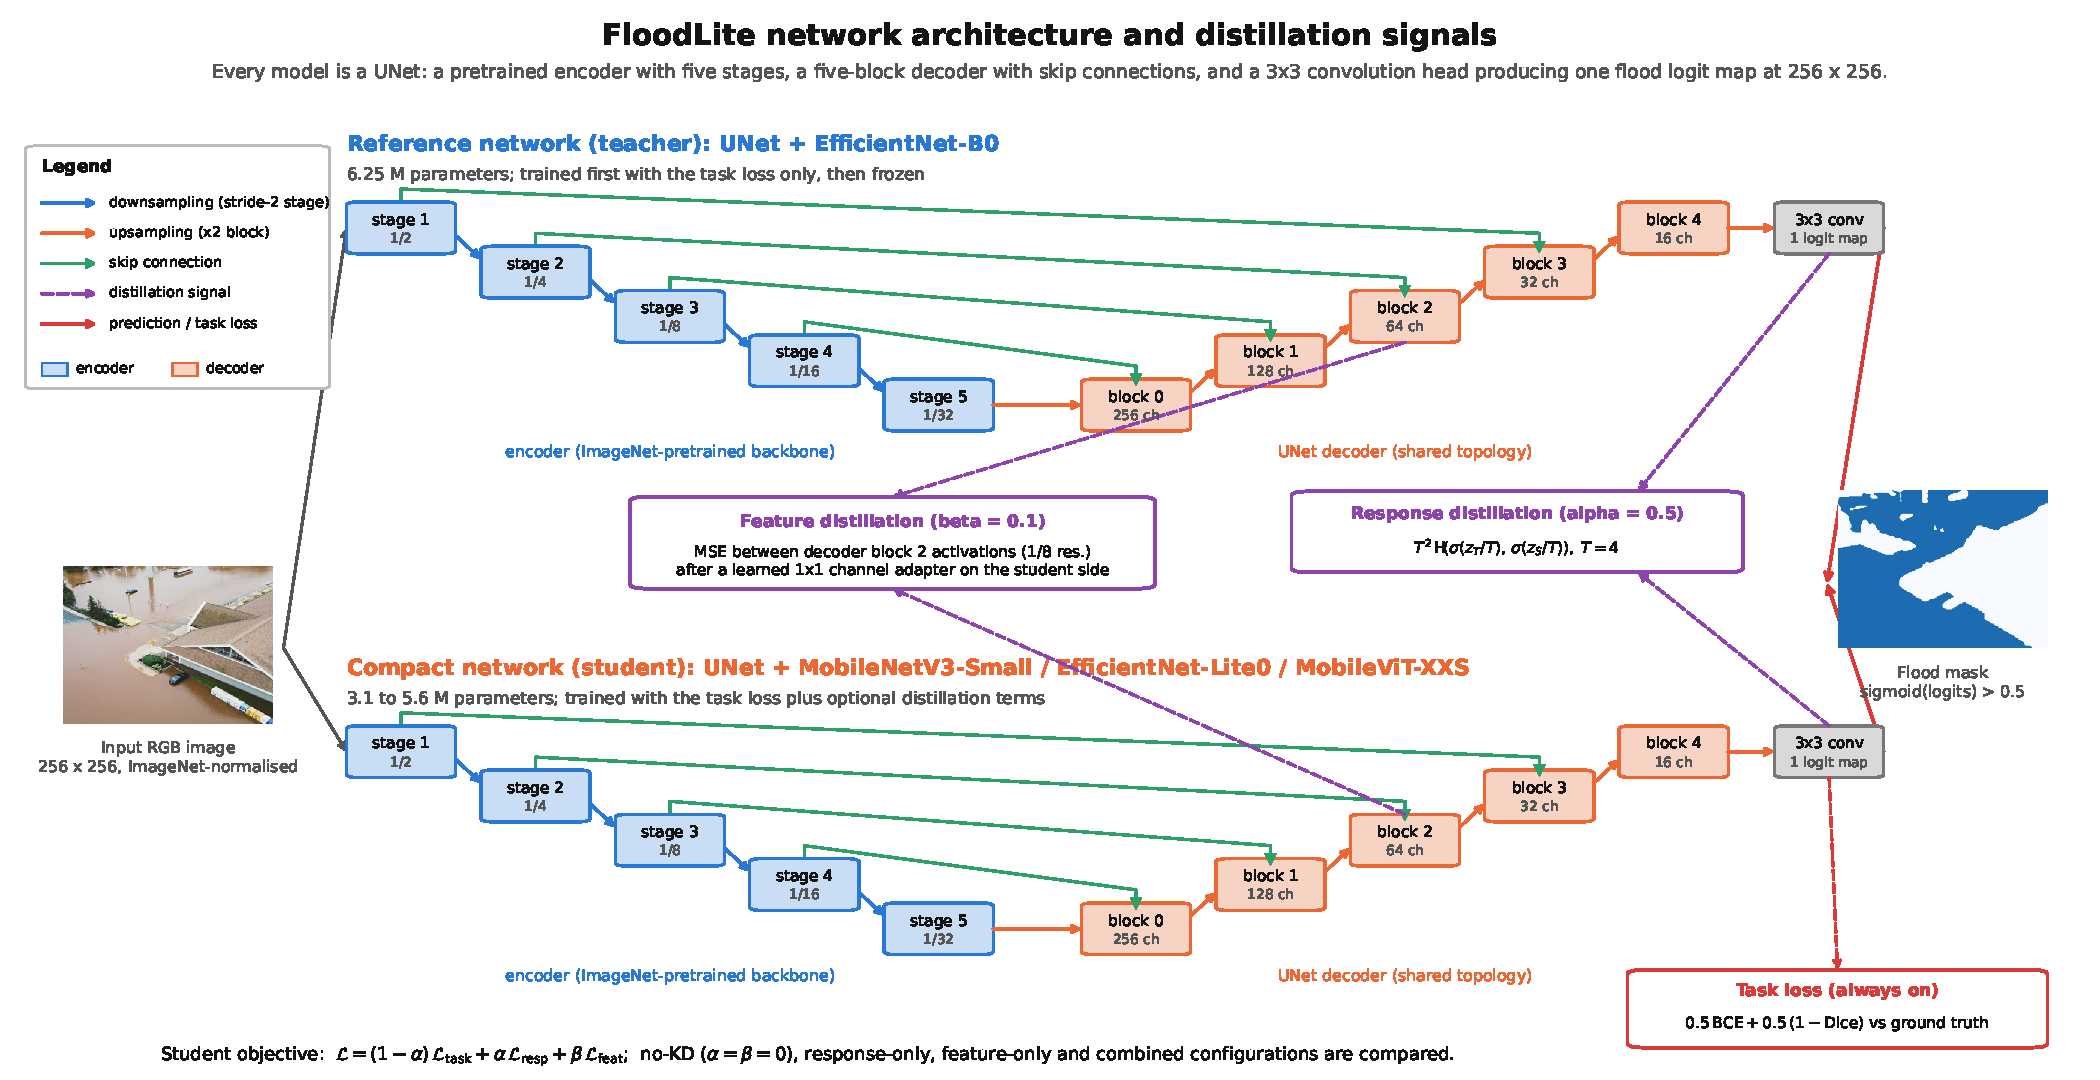
\includegraphics[width=0.98\linewidth]{figures/F6_architecture.pdf}
\caption{\textbf{Network architecture and distillation signals.} Every model is a UNet: a five-stage ImageNet-pretrained encoder, a five-block decoder (256/128/64/32/16 channels) with skip connections at matching resolution, and a $3{\times}3$ convolution head that outputs one logit map at $256{\times}256$. The reference network (top) uses an EfficientNet-B0 encoder, is trained with the task loss only and is then frozen. Each compact network (bottom) swaps in a MobileNetV3-Small, EfficientNet-Lite0 or MobileViT-XXS encoder and keeps the decoder topology. Response distillation compares the two logit maps at temperature $T=4$; feature distillation compares the decoder block~2 activations (1/8 resolution) through a learned $1{\times}1$ adapter on the compact network's side; the task loss (BCE $+$ Dice against the ground truth) is always applied.}
\label{fig:f6-architecture}
\end{figure*}

% =====================================================================
%  Table T1 -- Model Footprints
%  Source of truth: code/runs/3fold/summary.json + ONNX file sizes.
% =====================================================================
\begin{table}[ht]
\centering
\caption{\textbf{Model footprints.} Parameter counts from \texttt{torchinfo.summary}; GFLOPs at $256{\times}256$ (single image, multiply--adds counted as two FLOPs) from PyTorch's \texttt{FlopCounterMode}; ONNX disk sizes from the exported \texttt{.onnx} files. GFLOPs are dominated by the shared UNet decoder at this resolution, so they vary far less across backbones than parameter counts do.}
\label{tab:t1-footprints}
\footnotesize
\setlength{\tabcolsep}{4pt}
\begin{adjustbox}{max width=\textwidth}
\begin{tabular}{@{}lrrrr@{}}
\toprule
\textbf{Model} & \textbf{Params} & \textbf{GFLOPs} & \textbf{FP32} & \textbf{INT8} \\
               & \textbf{(M)}    & \textbf{(256\textsuperscript{2})} & \textbf{(MB)} & \textbf{(MB)} \\
\midrule
Teacher (UNet$+$EffB0)  & 6.25 & 5.92 & 22.3 & --  \\
MobileNetV2 baseline    & 6.63 & 6.69 & --  & --  \\
MobileNetV3-Small       & 3.59 & 5.11 & 13.8 & 3.7  \\
EfficientNet-Lite0      & 5.61 & 5.91 & 19.8 & 5.2  \\
MobileViT-XXS           & 3.09 & 5.43 & 12.0 & 3.5  \\
\bottomrule
\end{tabular}
\end{adjustbox}
\end{table}


\subsection{Knowledge distillation framework}
\label{sec:methods-kd}

We employ a two-component distillation loss as a controlled ablation, evaluated in three configurations, response-only ($\beta=0$, $\alpha=0.5$), feature-only ($\alpha=0$, $\beta=0.1$), and combined response $+$ feature ($\alpha=0.5$, $\beta=0.1$), against a no-KD baseline ($\alpha=0$, $\beta=0$). The KD configuration is treated as a categorical ablation variable rather than as a tuned hyperparameter; the formulation is the standard one (Hinton-style temperature-scaled binary cross-entropy on softened logits~\cite{hinton2015distilling} plus FitNet-style feature MSE on a matched decoder block through a $1{\times}1$ adapter~\cite{romero2015fitnets}), and the empirical question we ask is whether \emph{any} of $\{$response, feature, combined$\}$ confers a measurable benefit on this task.

Let $x \in \mathbb{R}^{H \times W \times 3}$ denote an input image, $y \in \{0,1\}^{H \times W}$ the ground-truth flood mask, $\hat{z}_T, \hat{z}_S \in \mathbb{R}^{H \times W}$ the pre-sigmoid logits produced by teacher and student respectively, and $f_T^{(\ell)}, f_S^{(\ell)}$ the activations at decoder stage $\ell$.

\paragraph{Task loss.} The per-pixel task loss combines binary cross-entropy and Dice:
\begin{equation}
\mathcal{L}_{\mathrm{task}} = 0.5 \cdot \mathrm{BCE}(\sigma(\hat{z}_S), y) + 0.5 \cdot \bigl(1 - \mathrm{Dice}(\sigma(\hat{z}_S), y)\bigr)
\label{eq:task}
\end{equation}
where $\sigma(\cdot)$ is the element-wise sigmoid.

\paragraph{Response-based distillation.} A temperature-scaled binary cross-entropy between the teacher's soft probabilities and the student's softened outputs (equal to the teacher--student KL divergence up to a teacher-only additive constant, and therefore yielding identical student gradients; this is what \texttt{floodlite/losses.py} computes):
\begin{equation}
\mathcal{L}_{\mathrm{resp}} = T^{2} \cdot \mathrm{H}\!\left(\sigma(\hat{z}_T / T),\;\sigma(\hat{z}_S / T)\right)
\label{eq:resp}
\end{equation}
where $\mathrm{H}(p,q) = -\,p\log q - (1-p)\log(1-q)$ is the element-wise binary cross-entropy and $T=4$ is the temperature. The $T^{2}$ factor preserves gradient magnitudes at increased temperatures~\cite{hinton2015distilling}.

\paragraph{Feature-based distillation.} We align student and teacher features at one matched decoder stage (resolution $64{\times}64$), introducing a $1{\times}1$ convolutional adapter $g_\theta$ to project student features into the teacher's channel space:
\begin{equation}
\mathcal{L}_{\mathrm{feat}} = \frac{1}{H \cdot W \cdot C_T} \bigl\| g_\theta\bigl(f_S^{(\ell)}\bigr) - f_T^{(\ell)} \bigr\|_{2}^{2}
\label{eq:feat}
\end{equation}

\paragraph{Combined loss.} The full FloodLite training objective:
\begin{equation}
\mathcal{L}_{\mathrm{FloodLite}} = (1 - \alpha) \cdot \mathcal{L}_{\mathrm{task}} + \alpha \cdot \mathcal{L}_{\mathrm{resp}} + \beta \cdot \mathcal{L}_{\mathrm{feat}}
\label{eq:combined}
\end{equation}
with $\alpha=0.5$ and $\beta=0.1$. The teacher is frozen during student training.

\subsection{Post-training INT8 quantization}
\label{sec:methods-ptq}

Post-training INT8 quantization (PTQ) is performed on the ONNX export of each student rather than on the PyTorch graph. This choice is forced by two practical findings during development. First, PyTorch eager-mode static PTQ requires CPU tensors for the calibration loop; the existing \texttt{floodlite/quantize.py} initially attempted CUDA calibration and failed. Second, even after fixing the device-placement bug, several \texttt{timm}-\allowbreak prefixed encoders (the \texttt{tf\_\allowbreak efficientnet\_\allowbreak lite0} and \texttt{mobilevit\_xxs} variants) use a \texttt{Conv2dSame} layer for which no quantized CPU kernel exists in PyTorch 2.7$+$. Quantization at the PyTorch graph level therefore cannot reach the full student set without modifying upstream \texttt{timm} source.

We instead use the ONNX Runtime \texttt{quantize\_static} API~\cite{ortQuant} (\texttt{onnxruntime.quantization}, v1.22.1), which operates on the ONNX graph and is independent of the upstream PyTorch operator set. The resulting INT8 QDQ graphs embed \texttt{ai.onnx.ml} opset~5 and therefore require ONNX Runtime~$\geq 1.18$ to load (ORT~1.17 cannot). Our recipe is:

\begin{enumerate}
\item \textbf{Pre-processing.} The FP32 ONNX is passed through \texttt{quant\_pre\_process} to fuse Conv-BN, fold constants, and lift the graph into a form that \texttt{quantize\_static} can analyse.
\item \textbf{Calibration.} We select 80 images (10 batches of 8) drawn only from the current fold's training split and never from the held-out validation images on which INT8 IoU is reported, run the FP32 graph against them through a custom \texttt{CalibrationDataReader} (\texttt{\_TorchLoaderCalibReader} in \texttt{floodlite/quantize.py}, invoked with \texttt{n\_calib\_batches=10} in \texttt{scripts/quantize\_all.py}), and record activation histograms.
\item \textbf{Quantization scheme.} Static QDQ (Quantize--DeQuantize) format with \emph{per-tensor} scales for both weights and activations (\texttt{per\_channel=False} in \texttt{floodlite/quantize.py}), with quantization restricted to \texttt{Conv}, \texttt{Gemm}, and \texttt{MatMul} operators via the \texttt{op\_types\_to\_quantize} argument. The op-type restriction leaves LayerNorm and elementwise \texttt{Add} operators in FP32. Per-tensor weights are the tool's default and are what Tables~\ref{tab:t4-quant}, \ref{tab:t9-zeroshot} and~\ref{tab:t11-combined-int8} report; Section~\ref{sec:results-quant} re-quantizes the FSSD no-KD students and the teacher with per-channel weights, with selected operators kept in FP32, and (on one fold) with unsigned activations, holding everything else fixed (\texttt{scripts/ptq\_mechanism\_ablation.py}, \texttt{scripts/ptq\_mobilevit\_diagnostic.py}).
\item \textbf{Calibration method.} We use \emph{Percentile} (99.999\%) rather than MinMax. MinMax is sensitive to single-image outlier activations on flood images with extreme reflective surfaces (wet asphalt, sun-glare on water), and produces unstable cross-fold INT8 IoU in our initial sweeps. Percentile-99.999\% is the most robust calibration option we evaluated and is the recipe we report in Section~\ref{sec:results-quant}.
\end{enumerate}

The resulting INT8 graph is consumed by ONNX Runtime's CPU execution provider; no ONNX\,$\rightarrow$\,TFLite or ONNX\,$\rightarrow$\,CoreML conversion is required, which is one motivation for our ONNX-centred deployment hub (Section~\ref{sec:methods-deploy}).

\subsection{Deployment pipeline}
\label{sec:methods-deploy}

Models are exported via PyTorch's TorchScript-based ONNX exporter (\texttt{torch.onnx.export} with \texttt{dynamo=False} and \texttt{opset\_version=13}) to a single \texttt{.onnx} file with embedded weights. We deliberately disable the PyTorch 2.8$+$ Dynamo exporter (\texttt{dynamo=True}) which produces separate \texttt{.data} sidecar files for weights; this complicates artifact distribution and is not yet uniformly supported across edge runtimes. The FP32 latency artifacts use opset 13; the static-QDQ INT8 path (Section~\ref{sec:methods-ptq}) re-exports and quantizes the same trained weights at opset 17, the default of the ONNX Runtime static-quantization tool. We did not time the FP32 graphs at opset 17, so FP32-versus-INT8 speed ratios carry this small confound.

Figure~\ref{fig:f8-inference} traces the inference path of the released code from an image file to a flood mask: resize to $256{\times}256$, ImageNet normalisation, one ONNX Runtime session call, a sigmoid with a 0.5 threshold, and a nearest-neighbour resize of the mask back to the input size. The six steps are the same on the CPU hosts and in the browser; only the runtime object differs.

\begin{figure*}[ht]
\centering
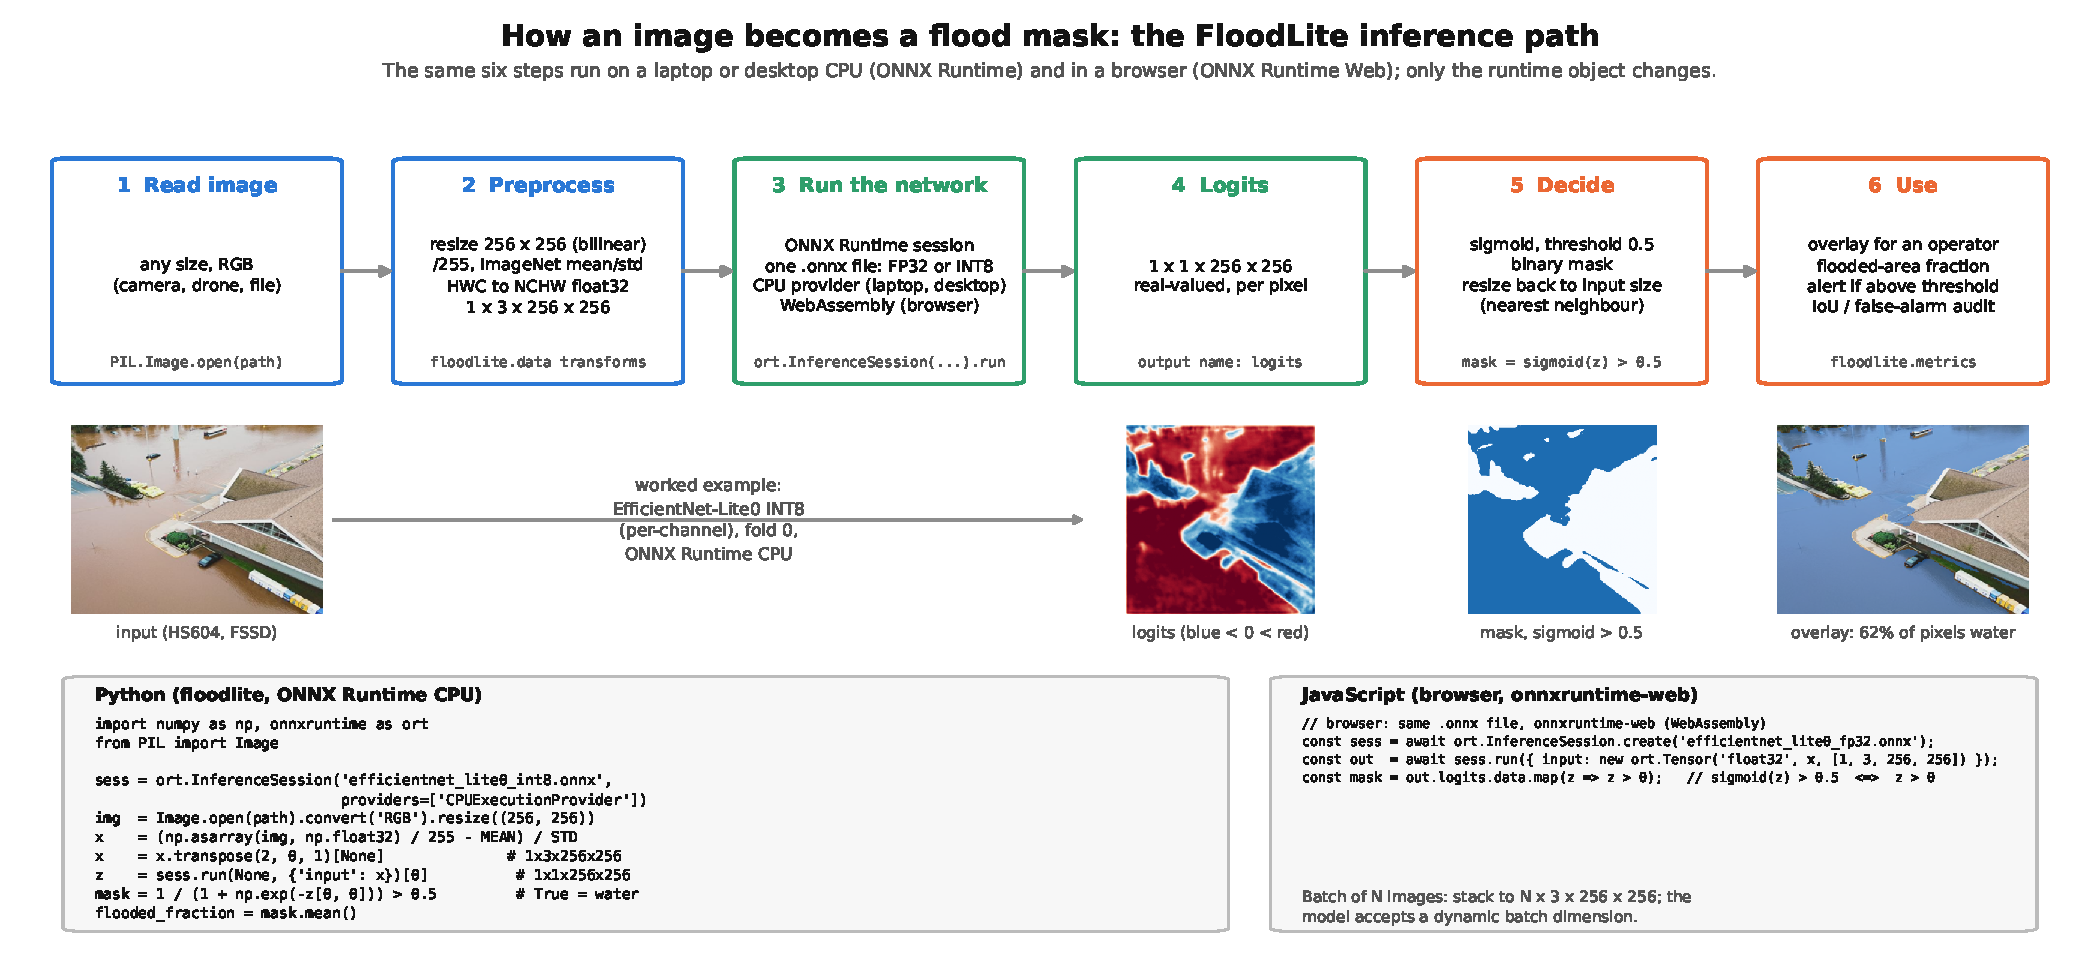
\includegraphics[width=0.98\linewidth]{figures/F8_inference_flow.pdf}
\caption{\textbf{How an image becomes a flood mask.} The six inference steps of the released code with tensor shapes and the calls that implement them, a worked example on an FSSD image using the EfficientNet-Lite0 INT8 export (per-channel recipe, fold 0) on ONNX Runtime CPU, and the Python and browser (ONNX Runtime Web) snippets. A positive logit is water; the model accepts a dynamic batch dimension.}
\label{fig:f8-inference}
\end{figure*}

We use ONNX as the single deployment hub. The same \texttt{.onnx} artifact serves both deployment targets in this paper:

\begin{itemize}
\item \textbf{Apple M2~Pro:} ONNX Runtime 1.22.1 with the \texttt{CPUExecutionProvider}. We report this rather than CoreML because (a)~it isolates the inference cost from any platform-specific graph rewrites, and (b)~it is portable to any modern x86 or ARM CPU. We did not benchmark CoreML or the Apple Neural Engine; ORT-CPU is the only M2 number reported.
\item \textbf{Browser:} ONNX Runtime Web 1.17 with the WebAssembly SIMD execution provider, single-threaded. We benchmark from Node.js~25 rather than from a Chrome page because (a)~in pilot runs that we did not archive, Chrome's WASM timings fell within $\pm 10\%$ of Node's, and (b)~it removes the SharedArrayBuffer / COOP--COEP browser configuration as a measurement-environment variable.
\item \textbf{Second host (x86):} an AMD Ryzen~5~5600G desktop under Windows~10, running the same ONNX Runtime 1.22.1 CPU execution provider natively (\texttt{scripts/bench\_ort\_cpu.py}) and ONNX Runtime Web 1.22.0 from Node.js~22 (\texttt{scripts/bench\_wasm\_node.mjs}), with the same warm-up and run counts. This host times the fold-0 artifacts of Section~\ref{sec:results-quant}, including the INT8 teacher, and is the only host on which INT8 artifacts could be loaded in the browser runtime.
\end{itemize}

INT8 latency is reported for the M2~Pro CPU target only. Our INT8 QDQ artifacts embed an operator-set version that requires ONNX Runtime $\geq 1.18$; ONNX Runtime Web 1.17.3 failed to load them (the failures are recorded in our supplementary \texttt{lat\_wasm.json}), so the WASM INT8 column of Table~\ref{tab:t5-latency} reads ``n/a''. A newer ORT-Web release may run them; we have not re-measured.

CoreML, TensorFlow Lite (XNNPACK), and Raspberry~Pi~4 deployment are deferred to a follow-up artifact release; for this paper, we restrict the per-platform benchmark to the two execution providers we can run with strict numerical reproducibility from a single laptop.

% =====================================================================
%  Section 4 -- Experimental Setup
% =====================================================================

\section{Experimental setup}
\label{sec:experimental-setup}

\subsection{Implementation}
\label{sec:setup-impl}

Training is implemented in PyTorch 2.8 with \texttt{segmentation-models-pytorch} 0.4~\cite{iakubovskii2019smp} for UNet decoder construction and \texttt{timm} 1.0~\cite{wightman2019timm} for backbone implementations. Mixed-precision (AMP fp16) training runs on a Kaggle Tesla T4 GPU (16\,GB) with batch size 8 (teacher) or 16 (students). Optimisation uses AdamW with learning rate $3\!\times\!10^{-4}$, weight decay $10^{-4}$, and a cosine schedule. Training runs for 35 epochs (teacher and students alike); empirically, validation IoU plateaus by epoch $\sim 25$. Data augmentation is provided by Albumentations~\cite{buslaev2020albumentations}: random horizontal flip, random rotation $\pm 15^{\circ}$, random brightness/contrast jitter ($\pm 0.2$), and ImageNet normalisation. The random seed is fixed at 42.

ONNX export, INT8 quantization, and CPU/WASM latency benchmarks run locally on an Apple M2~Pro (10-core CPU, 16\,GB unified memory, macOS 26.2); the quantization ablation and the second-host latencies (Section~\ref{sec:setup-latency}) run on an AMD Ryzen~5~5600G desktop (16\,GB, Windows~10). The Kaggle T4 is used for training only.

\subsection{Cross-validation protocol}
\label{sec:setup-cv}

We evaluate folds 0--2 of the five-fold partition \texttt{sklearn.\allowbreak{}model\_selection.\allowbreak{}KFold(n\_splits=5,\allowbreak\,shuffle=True,\allowbreak\,random\_state=42)} (Section~\ref{sec:methods-data} explains the reduction from five folds). The same fold indices are used for every $(\text{model} \times \text{KD configuration})$ combination, so all IoU comparisons in Tables~\ref{tab:t2-segmentation}--\ref{tab:t5-latency} are \emph{paired} across folds.

\subsection{Metrics}
\label{sec:setup-metrics}

We report pixel accuracy, precision, recall, F1-score, and mean intersection-over-union (IoU). For the within-regime zero-shot evaluation (Section~\ref{sec:results-zeroshot}) metrics are computed \emph{per image} and reported as macro statistics, since those test sets mix flood and flood-free scenes: an image with no water in the ground truth and none predicted counts as a correct rejection (IoU 1); over flood-containing images we report the flood-only IoU; and over water-free images we report the false-alarm rate (FAR), the fraction on which the model predicts any water at all. Efficiency metrics are model parameters (M, from \texttt{torchinfo.summary}) and ONNX disk size (MB). Latency is reported as median (p50), 95th percentile (p95), mean, and standard deviation over 200 timed forward passes after 20 warm-up passes; throughput as FPS $= 1000\,/\,\text{p50}_{\text{ms}}$. All latency measurements use single-image batches at $256{\times}256$ input resolution.

\subsection{Statistical validation}
\label{sec:setup-stats}

For each $(\text{model} \times \text{KD configuration})$, we report mean $\pm$ standard deviation across the 3 folds. The paired Wilcoxon signed-rank test is applied to the no-KD vs.~comb-KD contrast on each architecture, using fold-level paired IoU as the unit of observation; with $n=3$ folds its minimum reportable two-sided p-value is 0.25, so we treat it only as a coarse fold-level consistency check. For adequately-powered inference we additionally run a \emph{per-image paired bootstrap}: we pool per-image IoU over the held-out validation images of all three folds ($n=399$ images) and, for each contrast, resample images with replacement ($10{,}000$ replicates) to obtain a 95\% confidence interval on the mean paired IoU difference and a one-sided p-value (\texttt{scripts/stats\_bootstrap.py}; output archived as \texttt{runs/3fold/stats\_bootstrap.json}). Per-image IoU is a biased estimator of the pooled-pixel IoU of Table~\ref{tab:t2-segmentation} (small-flood images weigh as much as large ones), but the bias is image-specific and cancels in the \emph{paired} difference, which is the estimand. This bootstrap, not the three-fold Wilcoxon, supports the significance statements in Section~\ref{sec:results-kd}.

\subsection{Per-platform latency measurement}
\label{sec:setup-latency}

\begin{itemize}
\item \textbf{Apple M2~Pro / ONNX Runtime 1.22.1 CPU EP:} \texttt{scripts/bench\_m2.py}. Default ONNX Runtime CPU threading (the intra-op and inter-op thread counts are left at their defaults; the M2~Pro exposes up to 10 intra-op threads), matching realistic laptop deployment where all cores are available. 20 warm-up $+$ 200 timed runs.
\item \textbf{Browser WebAssembly SIMD / ONNX Runtime Web 1.17 from Node.js~25:} \texttt{bench.mjs} (supplementary). WASM execution provider with SIMD enabled and \texttt{numThreads} set to 1. 20 warm-up $+$ 200 timed runs. Equivalent in-browser numbers (Chrome 130, macOS 26.2) were verified to fall within $\pm 10\%$ in pilot runs.
\item \textbf{Second host, AMD Ryzen~5~5600G (6 cores, Windows~10):} \texttt{scripts/bench\_ort\_cpu.py} (ONNX Runtime 1.22.1 CPU EP, default threading) and \texttt{scripts/bench\_wasm\_node.mjs} (ONNX Runtime Web 1.22.0, WASM SIMD, one thread, Node.js~22), same warm-up and run counts. Timed on the fold-0 FP32 and INT8 artifacts produced by the quantization ablation (Section~\ref{sec:results-quant}), which are opset-17 exports; FP32 and INT8 are therefore compared at the same opset on this host.
\end{itemize}

All benchmarks consume the identical \texttt{.onnx} artifact; no platform-specific graph rewrites are performed.

% =====================================================================
%  Section 5 -- Results
% =====================================================================

\section{Results}
\label{sec:results}

This section is organised around Tables~\ref{tab:t1-footprints}--\ref{tab:t13-host2} and Figures~\ref{fig:f2-pareto}--\ref{fig:f4-throughput}. The pipeline schematic (Figure~\ref{fig:f1-pipeline}) is shown in Section~\ref{sec:methods} and the qualitative panel (Figure~\ref{fig:f3-qualitative}) in Section~\ref{sec:results-pipeline}.

\subsection{Teacher performance and comparison with Karc{\i} \emph{et al.}~(2026)}
\label{sec:results-teacher}

Our UNet $+$ EfficientNet-B0 teacher achieves \textbf{IoU $= \teacherIoU \pm \teacherStd$} on FSSD across the three folds (F1 $= 0.9611 \pm 0.0044$, accuracy $= 0.9729 \pm 0.0025$). The reference UNet $+$ EfficientNet-B7 number reported by Karc{\i} \emph{et al.}~\cite{karci2026deep} is IoU $= 0.927$, achieved with approximately $10\times$ the parameters ($\sim 63$\,M vs.~our 6.25\,M). The 0.0013 IoU gap between our B0 teacher and the published B7 reference is within the cross-fold standard deviation of both studies and indicates that the FSSD benchmark saturates well before the B7 capacity is required; B0 is sufficient as the teacher.

\subsection{Compact networks match or exceed the reference network without distillation}
\label{sec:results-kd}

The full segmentation results across all 14 configurations $\times$ 3 folds appear in Table~\ref{tab:t2-segmentation}. Three observations:

% =====================================================================
%  Table T2 -- In-Distribution Segmentation
%  Source of truth: code/runs/3fold/summary.json
% =====================================================================
\begin{table*}[ht]
\centering
\caption{\textbf{In-distribution segmentation performance.} Mean $\pm$ std over 3 folds (FSSD val, $256{\times}256$). Best per metric in \textbf{bold}.}
\label{tab:t2-segmentation}
\small
\setlength{\tabcolsep}{4pt}
\begin{adjustbox}{max width=\textwidth}
\begin{tabular}{lccccc}
\toprule
\textbf{Model / KD}                & \textbf{Acc}             & \textbf{Prec}            & \textbf{Rec}             & \textbf{F1}              & \textbf{IoU}             \\
\midrule
Teacher (UNet$+$EffB0)             & 0.9729 $\pm$ 0.0025      & 0.9623 $\pm$ 0.0077      & 0.9604 $\pm$ 0.0010      & 0.9611 $\pm$ 0.0044      & 0.9257 $\pm$ 0.0078      \\
MobileNetV2 baseline               & 0.9729 $\pm$ 0.0010      & 0.9632 $\pm$ 0.0052      & 0.9595 $\pm$ 0.0028      & 0.9611 $\pm$ 0.0019      & 0.9257 $\pm$ 0.0032      \\
\midrule
MobileNetV3-S / none               & 0.9732 $\pm$ 0.0006      & 0.9620 $\pm$ 0.0068      & 0.9620 $\pm$ 0.0050      & 0.9618 $\pm$ 0.0024      & 0.9269 $\pm$ 0.0043      \\
MobileNetV3-S / resp               & 0.9719 $\pm$ 0.0007      & 0.9599 $\pm$ 0.0050      & 0.9598 $\pm$ 0.0049      & 0.9596 $\pm$ 0.0016      & 0.9229 $\pm$ 0.0028      \\
MobileNetV3-S / feat               & 0.9732 $\pm$ 0.0012      & 0.9616 $\pm$ 0.0040      & 0.9626 $\pm$ 0.0025      & 0.9619 $\pm$ 0.0020      & 0.9271 $\pm$ 0.0035      \\
MobileNetV3-S / comb               & 0.9723 $\pm$ 0.0019      & 0.9603 $\pm$ 0.0062      & 0.9608 $\pm$ 0.0024      & 0.9604 $\pm$ 0.0034      & 0.9242 $\pm$ 0.0061      \\
\midrule
EfficientNet-Lite0 / none          & 0.9735 $\pm$ 0.0012      & 0.9654 $\pm$ 0.0048      & 0.9595 $\pm$ 0.0034      & 0.9622 $\pm$ 0.0026      & 0.9277 $\pm$ 0.0047      \\
EfficientNet-Lite0 / resp          & 0.9729 $\pm$ 0.0013      & 0.9622 $\pm$ 0.0037      & 0.9601 $\pm$ 0.0028      & 0.9609 $\pm$ 0.0007      & 0.9253 $\pm$ 0.0011      \\
EfficientNet-Lite0 / feat          & 0.9734 $\pm$ 0.0008      & 0.9654 $\pm$ 0.0054      & 0.9593 $\pm$ 0.0044      & 0.9621 $\pm$ 0.0020      & 0.9275 $\pm$ 0.0034      \\
EfficientNet-Lite0 / comb          & 0.9733 $\pm$ 0.0016      & 0.9633 $\pm$ 0.0051      & 0.9601 $\pm$ 0.0019      & 0.9615 $\pm$ 0.0021      & 0.9264 $\pm$ 0.0037      \\
\midrule
MobileViT-XXS / none               & \textbf{0.9771 $\pm$ 0.0023} & \textbf{0.9695 $\pm$ 0.0040} & \textbf{0.9650 $\pm$ 0.0025} & \textbf{0.9671 $\pm$ 0.0031} & \textbf{0.9367 $\pm$ 0.0055} \\
MobileViT-XXS / resp               & 0.9757 $\pm$ 0.0019      & 0.9659 $\pm$ 0.0055      & 0.9642 $\pm$ 0.0016      & 0.9649 $\pm$ 0.0033      & 0.9326 $\pm$ 0.0060      \\
MobileViT-XXS / feat               & 0.9766 $\pm$ 0.0014      & 0.9680 $\pm$ 0.0051      & 0.9655 $\pm$ 0.0039      & 0.9665 $\pm$ 0.0026      & 0.9357 $\pm$ 0.0046      \\
MobileViT-XXS / comb               & 0.9752 $\pm$ 0.0025      & 0.9657 $\pm$ 0.0053      & 0.9636 $\pm$ 0.0025      & 0.9644 $\pm$ 0.0039      & 0.9318 $\pm$ 0.0070      \\
\bottomrule
\end{tabular}
\end{adjustbox}
\end{table*}


\begin{enumerate}
\item \textbf{MobileViT-XXS without distillation is the most accurate network of all.} In the no-KD configuration it attains IoU $= \bestStudentIoU \pm \bestStudentStd$, \emph{0.011 IoU points above the teacher} (\teacherIoU $\pm$ \teacherStd). The student is also $2.0\times$ smaller in parameters (3.09\,M vs.~6.25\,M). This is the headline result against which the original KD-recipe framing of this paper has to be evaluated.
\item \textbf{EfficientNet-Lite0 (no-KD) matches the teacher within standard deviation} ($0.9277 \pm 0.0047$ vs.~$\teacherIoU \pm \teacherStd$). MobileNetV3-Small (no-KD) likewise matches it ($0.9269 \pm 0.0043$).
\item \textbf{The MobileNetV2 baseline also matches the teacher} ($0.9257 \pm 0.0032$). An off-the-shelf lightweight encoder of the same size class (6.6\,M vs.\ 6.3\,M parameters, Table~\ref{tab:t1-footprints}) therefore does as well as the teacher; the teacher is itself a lightweight UNet, not a ``heavy'' model in the regime where KD typically helps.
\end{enumerate}

We interpret these observations as direct evidence that FSSD, at 663 RGB images and IoU $\approx 0.93$, is saturated for the ImageNet-pretrained UNet family. The variance across $(\text{model} \times \text{KD})$ cells of Table~\ref{tab:t2-segmentation} is dominated by fold-level seed noise rather than by genuine architectural separations. KD has no headroom to transfer.

Table~\ref{tab:t3-kd-ablation} isolates the KD ablation on the best student. None of the three KD configurations improves on the no-KD baseline:

% =====================================================================
%  Table T3 -- KD Ablation on Best Student
%  Source of truth: code/runs/3fold/summary.json + stats.json (Wilcoxon)
% =====================================================================
\begin{table}[ht]
\centering
\caption{\textbf{KD ablation on the best student (MobileViT-XXS).} Wilcoxon two-sided; $n=3$ folds gives a minimum reportable $p \approx 0.25$. $\Delta$IoU is relative to no KD.}
\label{tab:t3-kd-ablation}
\small
\setlength{\tabcolsep}{4pt}
\begin{adjustbox}{max width=\textwidth}
\begin{tabular}{lccc}
\toprule
\textbf{KD} & \textbf{IoU (mean $\pm$ std)} & \textbf{$\Delta$IoU} & \textbf{Wilcoxon $p$} \\
\midrule
none      & 0.9367 $\pm$ 0.0055 & --      & -- \\
resp      & 0.9326 $\pm$ 0.0060 & $-0.0041$ & n/a \\
feat      & 0.9357 $\pm$ 0.0046 & $-0.0011$ & n/a \\
comb      & 0.9318 $\pm$ 0.0070 & $-0.0049$ & 0.250 \\
\bottomrule
\end{tabular}
\end{adjustbox}
\end{table}


The Wilcoxon test on no-KD vs.~comb-KD yields $p = 0.250$, the minimum two-sided p-value reportable at $n=3$, which means the fold-level test is consistent with both ``comb-KD is no worse'' and ``comb-KD is meaningfully worse'' under low power, but in no case does it support ``comb-KD is better''. Across \emph{all three architectures $\times$ three KD configurations $\times$ three folds}, the combined KD configuration produces a higher mean IoU than the no-KD baseline in zero out of three architectures.

Beyond the fold-level means, the \emph{direction} of the effect is consistent: for the best student, MobileViT-XXS, the combined-KD IoU is below the no-KD IoU in every one of the three folds, and the no-KD MobileViT-XXS exceeds the teacher in every fold (fold-wise margins $+0.013$, $+0.016$, $+0.004$ IoU; mean $+0.011$).

The per-image paired bootstrap (Section~\ref{sec:setup-stats}; $n=399$ held-out validation images, $10{,}000$ replicates; archived as \texttt{runs/3fold/stats\_bootstrap.json}) sharpens this into a powered statement. Across all nine (architecture $\times$ KD-configuration) contrasts, \emph{no} KD configuration significantly improves over its no-KD baseline: no 95\% confidence interval on $\Delta\mathrm{IoU}_{\text{no-KD}-\text{KD}}$ lies entirely below zero. Two contrasts show KD significantly \emph{worse} after Holm correction for the nine comparisons (one-sided bootstrap $p$): response-only KD on MobileViT-XXS ($\Delta = +0.0065$, 95\% CI $[+0.0029,+0.0103]$, $p=0.0001$) and combined KD on MobileViT-XXS ($+0.0076$, $[+0.0035,+0.0118]$, $p=0.0002$). Response-only KD on MobileNetV3-Small ($+0.0047$, $[+0.0008,+0.0091]$, $p=0.010$) and on EfficientNet-Lite0 ($+0.0040$, $[-0.0007,+0.0086]$, $p=0.046$) point the same way but do not survive the correction; the remaining five contrasts show no effect. The response-based term is therefore harmful for MobileViT-XXS and borderline for the other two, consistent with its interpretation as a noise-injection regulariser on a saturated benchmark (Section~\ref{sec:discussion-negative-kd}). The headline result is likewise significant: MobileViT-XXS (no-KD) exceeds the teacher by $\Delta\mathrm{IoU} = +0.015$ per image (95\% CI $[+0.010,+0.020]$, $p < 0.001$).

\subsection{INT8 quantization: a recipe artefact for the CNNs, a real loss for MobileViT}
\label{sec:results-quant}

Table~\ref{tab:t4-quant} summarises post-training INT8 quantization of the three students under the per-tensor recipe of Section~\ref{sec:methods-ptq}:

% =====================================================================
%  Table T4 -- Quantization
%  Source of truth: code/runs/3fold/quantized.json + ONNX file sizes.
% =====================================================================
\begin{table*}[ht]
\centering
\caption{\textbf{Post-training INT8 quantization under the per-tensor recipe} (static QDQ, per-tensor weight and activation scales, Percentile-99.999\% calibration, 80 train images). EfficientNet-Lite0 (highlighted) is the recommended deployable configuration; the other two students collapse under this recipe. For the two collapsing students the INT8 IoU is strongly multi-modal across folds (MobileNetV3-Small: $0.772 / 0.0001 / 0.657$; MobileViT-XXS: $0.718 / 0.464 / 0.244$), so their mean\,$\pm$\,std is an instability indicator, not a central tendency. Table~\ref{tab:t12-ptq-mechanism} shows that per-channel weight scales remove the MobileNetV3-Small collapse and most of the MobileViT-XXS loss comes from its early convolutions (Section~\ref{sec:results-quant}).}
\label{tab:t4-quant}
\small
\setlength{\tabcolsep}{4pt}
\begin{adjustbox}{max width=\textwidth}
\begin{tabular}{lcccccc}
\toprule
& & & & \multicolumn{2}{c}{\textbf{ONNX size (MB)}} & \\
\cmidrule(lr){5-6}
\textbf{Model} & \textbf{FP32 IoU} & \textbf{INT8 IoU} & \textbf{$\Delta$ IoU} & \textbf{FP32} & \textbf{INT8} & \textbf{Reduction} \\
\midrule
MobileNetV3-Small   & 0.9269 $\pm$ 0.0043 & 0.4762 $\pm$ 0.3399 & $-0.4507$ & 13.8 & 3.7 & $3.69\times$ \\
\textbf{EfficientNet-Lite0} & \textbf{0.9277 $\pm$ 0.0047} & \textbf{0.8851 $\pm$ 0.0149} & $\boldsymbol{-0.0426}$ & \textbf{19.8} & \textbf{5.2} & $\boldsymbol{3.83\times}$ \\
MobileViT-XXS       & 0.9367 $\pm$ 0.0055 & 0.4752 $\pm$ 0.1936 & $-0.4616$ & 12.0 & 3.5 & $3.42\times$ \\
\bottomrule
\end{tabular}
\end{adjustbox}
\end{table*}


Under an identical Percentile-99.999\% static QDQ recipe, EfficientNet-Lite0 retains 95\% of its FP32 IoU with a tight $\pm 0.015$ cross-fold standard deviation, whereas MobileNetV3-Small and MobileViT-XXS both lose $\sim 0.45$ IoU with cross-fold standard deviations of 0.19--0.34, an order of magnitude larger than EfficientNet-Lite0's. An earlier draft of this paper attributed the two collapses to the architectures, to MobileNetV3-Small's unbounded HardSwish activations and to MobileViT-XXS's attention and LayerNorm blocks. A controlled ablation (Table~\ref{tab:t12-ptq-mechanism}; \texttt{scripts/ptq\_mechanism\_ablation.py}) shows that this attribution was wrong for the first and incomplete for the second. For each fold the ablation shares the FP32 export, the 80 calibration images and the activation calibration, and changes one thing at a time; it also quantizes the teacher, which Table~\ref{tab:t4-quant} did not.

% =====================================================================
%  Table T12 -- PTQ mechanism ablation (per-tensor vs per-channel weights)
%  Source of truth: code/runs/3fold/ptq_mechanism.json
%  Producer: code/scripts/ptq_mechanism_ablation.py (ONNX Runtime 1.22.1)
%  Layer-group diagnostic (text): code/runs/3fold/ptq_mobilevit_groups.json
% =====================================================================
\begin{table*}[ht]
\centering
\caption{\textbf{What causes the INT8 collapse.} Change in IoU from FP32 to INT8 for the FSSD no-KD students and the teacher, folds 0\,/\,1\,/\,2 and mean\,$\pm$\,std. All variants share each fold's FP32 export (opset 17), the same 80 calibration images and the Percentile-99.999\% activation calibration, and differ only as stated. \emph{Per-tensor} is the recipe of Table~\ref{tab:t4-quant}, re-run under ONNX Runtime 1.22.1. \emph{Per-channel} changes only the weight scales. \emph{HardSwish FP32} additionally keeps the 15 Conv nodes fed by a HardSwish or hard-sigmoid output in FP32. \emph{Attention FP32} quantizes only Conv and leaves every MatMul (attention and MLP) in FP32. \emph{Early Convs FP32} keeps the stem and the first two encoder stages in FP32 and quantizes everything else, attention included. A dash means the variant does not apply to that model.}
\label{tab:t12-ptq-mechanism}
\small
\setlength{\tabcolsep}{4pt}
\begin{adjustbox}{max width=\textwidth}
\begin{tabular}{lccccc}
\toprule
& & & \multicolumn{3}{c}{\textbf{Per-channel, plus \ldots{} kept in FP32}} \\
\cmidrule(lr){4-6}
\textbf{Model} & \textbf{Per-tensor} & \textbf{Per-channel} & \textbf{HardSwish} & \textbf{Attention} & \textbf{Early Convs} \\
\midrule
MobileNetV3-Small & $-0.185 / -0.921 / -0.224$ & $-0.017 / -0.030 / -0.022$ & $-0.014 / -0.028 / -0.020$ & -- & -- \\
                  & $-0.444 \pm 0.338$ & $\mathbf{-0.023 \pm 0.006}$ & $-0.021 \pm 0.006$ & & \\
\addlinespace
EfficientNet-Lite0 & $-0.023 / -0.023 / -0.047$ & $-0.020 / -0.043 / -0.015$ & -- & -- & -- \\
                   & $-0.031 \pm 0.011$ & $-0.026 \pm 0.012$ & & & \\
\addlinespace
MobileViT-XXS     & $-0.223 / -0.402 / -0.921$ & $-0.219 / -0.237 / -0.330$ & -- & $-0.218 / -0.231 / -0.368$ & $-0.024 / -0.087 / -0.187$ \\
                  & $-0.515 \pm 0.296$ & $-0.262 \pm 0.049$ & & $-0.272 \pm 0.068$ & $-0.099 \pm 0.067$ \\
\addlinespace
Teacher (UNet$+$EffB0) & $-0.296 / -0.185 / -0.193$ & $-0.008 / -0.004 / -0.015$ & -- & -- & -- \\
                       & $-0.225 \pm 0.050$ & $\mathbf{-0.009 \pm 0.004}$ & & & \\
\bottomrule
\end{tabular}
\end{adjustbox}
\end{table*}


Four results follow.

\begin{enumerate}
\item \textbf{The per-tensor collapses reproduce, and the teacher collapses too.} Re-run under ONNX Runtime 1.22.1, the per-tensor recipe gives the same fold pattern as Table~\ref{tab:t4-quant}, including the fold-1 MobileNetV3-Small collapse to IoU 0.0001. The teacher, a UNet$+$EfficientNet-B0 with SiLU activations and squeeze-and-excitation gates, loses 0.19--0.30 IoU under the same recipe. The failure is therefore not specific to HardSwish or to attention: of the four networks, only EfficientNet-Lite0 survives per-tensor weight scales.
\item \textbf{Per-channel weight scales fix every convolutional network.} Changing only the weight quantizer from per-tensor to per-channel brings MobileNetV3-Small to $-0.023 \pm 0.006$ IoU and the teacher to $-0.009 \pm 0.004$, with no collapse in any fold; EfficientNet-Lite0 is unchanged ($-0.026 \pm 0.012$). This is the textbook remedy for depthwise convolutions, whose per-output-channel weight ranges differ by orders of magnitude~\cite{krishnamoorthi2018quantizing}, and it was the recipe setting we had left at its default. Keeping the 15 HardSwish-fed convolutions of MobileNetV3-Small in FP32 on top of per-channel scales gains a further 0.002 IoU, so the measured HardSwish activation range (maximum $156.7$ against EfficientNet-Lite0's ReLU6 ceiling of $6.0$; \texttt{scripts/ptq\_activation\_diagnostic.py}) is real but is not what broke the model. We retain the per-tensor numbers of Table~\ref{tab:t4-quant} because they are what the default ONNX Runtime tutorial produces, and because the deployment and zero-shot results of Sections~\ref{sec:results-latency}--\ref{sec:results-combined} were obtained with those artifacts.
\item \textbf{MobileViT-XXS loses 0.22--0.33 IoU under every full-quantization recipe, and its attention blocks are not the cause.} Per-channel scales reduce its loss from $-0.515 \pm 0.296$ to $-0.262 \pm 0.049$, removing the fold-dependence but not the loss. Keeping every \texttt{MatMul} (attention and MLP) in FP32 changes nothing ($-0.272 \pm 0.068$). A layer-group diagnostic (\texttt{scripts/ptq\_mobilevit\_diagnostic.py}, per-channel, one group quantized at a time with the rest FP32) locates the loss in the convolutional trunk \emph{before} the first transformer block: quantizing only the stem costs at most 0.002 IoU, only stage~0 costs 0.03--0.05, and only stage~1 costs 0.12--0.20, while quantizing only a transformer stage, the downsampling block of stage~3, or the decoder costs under 0.003 (fold~0). Keeping the stem and stages~0--1 in FP32 and quantizing everything else, attention included, leaves $-0.024 / -0.087 / -0.187$ IoU across the three folds (Table~\ref{tab:t12-ptq-mechanism}, last column), so these early high-resolution blocks carry most but not all of the damage, and the remainder is fold-dependent. We did not find a recipe that quantizes MobileViT-XXS to within 0.05 IoU of FP32 in every fold.
\item \textbf{Activation signedness does not matter for accuracy.} Re-quantizing the fold-0 models with unsigned 8-bit activations (the layout ONNX Runtime's x86 kernels prefer; Section~\ref{sec:results-latency}) changes IoU by at most $-0.010$ for the three convolutional networks and $-0.023$ for MobileViT-XXS relative to the signed per-channel artifacts (\texttt{runs/host2/u8s8\_fold0.json}).
\end{enumerate}

The practical implication: \emph{the INT8 collapse that a practitioner sees from the default ONNX Runtime static-quantization recipe is, for convolutional backbones, a per-tensor-weight artefact that per-channel scales remove; MobileViT-XXS is the exception, and the problem sits in its early convolutions rather than in attention.} We did not test quantization-aware training, which is the natural next step for MobileViT-XXS and an order-of-magnitude larger training investment. Section~\ref{sec:results-latency} shows that the fixed INT8 models are only worth deploying on hardware where INT8 is actually faster.

\subsection{Per-platform inference latency}
\label{sec:results-latency}

Table~\ref{tab:t5-latency} reports inference latency on the two deployment platforms of the main benchmark, and Table~\ref{tab:t13-host2} on a second, x86 host.

% =====================================================================
%  Table T5 -- Per-Platform Latency
%  Source of truth: code/runs/3fold/{lat_m2,lat_wasm}.json
% =====================================================================
\begin{table*}[ht]
\centering
\caption{\textbf{Per-platform inference latency.} Single-image batches, $256{\times}256$ input. M2~Pro and browser WASM both consume the same \texttt{.onnx} artifact under different execution providers. INT8 WASM rows are n/a on this host: our INT8 QDQ artifacts require ONNX Runtime $\geq 1.18$, and ONNX Runtime Web 1.17.3 failed to load them; Table~\ref{tab:t13-host2} measures them under ORT-Web 1.22.0 on a second host. \textsuperscript{a}Teacher timed under the same ONNX Runtime CPU execution provider as the students, under ORT 1.17 (37.6\,ms p50; 36.7\,ms when re-timed under the students' ORT 1.22.1). Under PyTorch eager CPU the same teacher is 274\,ms ($7.3\times$ slower); reporting that PyTorch figure against ORT-CPU students would inflate the apparent teacher-vs-student speedup. On a common ORT-CPU backend the FP32 students are only $1.1$--$1.9\times$ faster than the teacher, and the recommended EfficientNet-Lite0 INT8 is $2.2\times$ faster. The INT8 teacher of Table~\ref{tab:t12-ptq-mechanism} was not timed on this host. All timing rows trace to \texttt{lat\_m2.json} (student rows via \texttt{bench\_m2.py}; teacher ORT-CPU row via \texttt{bench\_teacher\_ort.py}); see \texttt{runs/3fold/PROVENANCE.md}.}
\label{tab:t5-latency}
\small
\setlength{\tabcolsep}{5pt}
\begin{adjustbox}{max width=\textwidth}
\begin{tabular}{lcccccc}
\toprule
\multirow{2}{*}{\textbf{Model}}
  & \multicolumn{3}{c}{\textbf{Apple M2~Pro (ORT-CPU)}}
  & \multicolumn{3}{c}{\textbf{Browser WASM SIMD (ORT-Web)}} \\
\cmidrule(lr){2-4} \cmidrule(lr){5-7}
  & p50 (ms) & p95 (ms) & FPS  & p50 (ms) & p95 (ms) & FPS  \\
\midrule
Teacher (UNet$+$EffB0) FP32\textsuperscript{a} & 37.6 & 44.2 & 26.6 & \multicolumn{3}{c}{n/a (out-of-scope for browser deploy)} \\
\midrule
MobileNetV3-Small FP32             &  19.5 &  20.4 & 51.2  & 133.3 & 134.8 & 7.5 \\
MobileNetV3-Small INT8             &  13.7 &  14.1 & 72.9  & \multicolumn{3}{c}{n/a (ORT-Web 1.17 limitation)} \\
EfficientNet-Lite0 FP32            &  34.2 &  52.7 & 29.3  & 163.8 & 210.5 & 6.1 \\
\textbf{EfficientNet-Lite0 INT8}   &  \textbf{17.3} & \textbf{20.1} & \textbf{57.7} & \multicolumn{3}{c}{n/a (ORT-Web 1.17 limitation)} \\
MobileViT-XXS FP32                 &  28.3 &  32.8 & 35.4  & 149.4 & 159.8 & 6.7 \\
MobileViT-XXS INT8                 &  21.6 &  25.0 & 46.3  & \multicolumn{3}{c}{n/a (ORT-Web 1.17 limitation)} \\
\bottomrule
\end{tabular}
\end{adjustbox}
\end{table*}


Three remarks on the Apple-Silicon host. First, the teacher-versus-student latency comparison must be read on a common runtime. Measured under the ONNX Runtime CPU backend, the teacher runs at 37.6\,ms p50 (26.6\,FPS; ORT 1.17, re-timed at 36.7\,ms under the students' ORT 1.22.1), not the 274\,ms of PyTorch eager mode; the PyTorch\,$\rightarrow$\,ORT switch alone is a $7.3\times$ speedup with no architecture change. On this common runtime the FP32 students are only $1.1$--$1.9\times$ faster than the teacher, so the deployment advantage of the recommended EfficientNet-Lite0 comes primarily from INT8 precision (a $2.2\times$ speedup over the teacher, 17.3 vs 37.6\,ms) and from its smaller binary, not from an FP32 latency gap. Second, \emph{INT8 yields a further $1.3$--$2.0\times$ speedup on top of the FP32 student baseline} on this ARM CPU. Third, \emph{the WASM column is $4.8$--$6.8\times$ slower than the M2-CPU column for the same FP32 model}, which is the expected single-threaded-WebAssembly-vs-native-CPU gap and represents an effective lower bound on browser-deployment performance. INT8 WASM rows are marked n/a because ONNX Runtime Web 1.17.3 could not load the INT8 artifacts (Section~\ref{sec:methods-deploy}).

% =====================================================================
%  Table T13 -- Second-host latency (x86 desktop): native ORT-CPU and
%  browser WASM, FP32 vs INT8, including the INT8 teacher.
%  Source of truth: code/runs/host2/{lat_ort_cpu,lat_wasm_node,lat_ort_cpu_u8s8}.json
%  Producers: scripts/bench_ort_cpu.py, scripts/bench_wasm_node.mjs
% =====================================================================
\begin{table*}[ht]
\centering
\caption{\textbf{Latency on a second host (AMD Ryzen~5~5600G desktop, Windows~10).} Fold-0 ONNX artifacts of the per-channel INT8 recipe (Table~\ref{tab:t12-ptq-mechanism}); p50 over 200 timed runs after 20 warm-ups, $1{\times}3{\times}256{\times}256$ input, same protocol as Table~\ref{tab:t5-latency}. Native: ONNX Runtime 1.22.1 CPU execution provider, default threads. Browser: ONNX Runtime Web 1.22.0, WebAssembly SIMD, one thread, from Node.js~22; this runtime loads every INT8 artifact that ORT-Web 1.17.3 rejected. \emph{INT8 speed-up} is FP32 p50 divided by INT8 p50 (values below 1 mean INT8 is slower). Per-tensor INT8 artifacts time within 2\% of the per-channel ones (\texttt{lat\_ort\_cpu.json}); INT8 with unsigned activations is 7--27\% faster than the signed-activation artifacts natively but still 2.2--2.6$\times$ slower than FP32 (\texttt{lat\_ort\_cpu\_u8s8.json}).}
\label{tab:t13-host2}
\small
\setlength{\tabcolsep}{4pt}
\begin{adjustbox}{max width=\textwidth}
\begin{tabular}{lcccccc}
\toprule
\multirow{2}{*}{\textbf{Model}}
  & \multicolumn{3}{c}{\textbf{Native x86 (ORT-CPU 1.22.1)}}
  & \multicolumn{3}{c}{\textbf{Browser WASM SIMD (ORT-Web 1.22.0)}} \\
\cmidrule(lr){2-4} \cmidrule(lr){5-7}
  & FP32 p50 (ms) & INT8 p50 (ms) & INT8 speed-up & FP32 p50 (ms) & INT8 p50 (ms) & INT8 speed-up \\
\midrule
Teacher (UNet$+$EffB0)   & 23.4 & 70.1 & $0.33\times$ & 225.4 & 178.7 & $1.26\times$ \\
MobileNetV3-Small        & 15.4 & 45.2 & $0.34\times$ & 173.9 & 122.7 & $1.42\times$ \\
EfficientNet-Lite0       & 16.8 & 46.3 & $0.36\times$ & 227.3 & 175.5 & $1.30\times$ \\
MobileViT-XXS            & 21.6 & 65.7 & $0.33\times$ & 199.2 & 152.8 & $1.30\times$ \\
\bottomrule
\end{tabular}
\end{adjustbox}
\end{table*}


The second host (Table~\ref{tab:t13-host2}; AMD Ryzen~5~5600G, Windows~10) adds the INT8 teacher, closes the browser INT8 gap, and reverses one conclusion. In the browser, ONNX Runtime Web 1.22.0 loads every INT8 artifact and runs it $1.26$--$1.42\times$ faster than FP32; per-channel INT8 MobileNetV3-Small reaches 8.2\,FPS at 3.8\,MB and IoU 0.904, the fastest and smallest browser configuration we measured. Natively, however, \emph{INT8 is $2.8$--$3.0\times$ slower than FP32 on this x86 CPU} for all four networks, under the same ONNX Runtime 1.22.1 CPU execution provider that gives a $1.3$--$2.0\times$ INT8 speedup on the M2~Pro. Switching the activations to the unsigned layout that ONNX Runtime's x86 kernels prefer recovers only 7--27\%, leaving INT8 $2.2$--$2.6\times$ slower than FP32. We have not established the cause; the processor lacks the AVX-512 VNNI instructions that accelerate 8-bit dot products, and the QDQ graphs may be falling back to de-quantized execution for some operators. Whatever the mechanism, the practical reading is that \emph{the INT8 speedup is a property of the CPU and runtime, not of the model}: the same artifact is $2\times$ faster than FP32 on one commodity CPU, $1.3\times$ faster in the browser, and $3\times$ slower on another commodity CPU. On the x86 host the best native configurations are FP32 MobileNetV3-Small (15.4\,ms, 65\,FPS) and FP32 EfficientNet-Lite0 (16.8\,ms), and the teacher itself runs at 23.4\,ms, only $1.1$--$1.5\times$ slower than the students. INT8 remains worthwhile there only for its $3.4$--$3.8\times$ smaller files.

\subsection{Pareto analysis}
\label{sec:results-pareto}

\begin{figure*}[ht]
\centering
\includegraphics[width=0.75\linewidth]{figures/F5_bubble.pdf}
\caption{\textbf{Consolidated accuracy--latency--size--precision trade-off.} Each configuration is placed by Apple~M2~Pro ORT-CPU p50 latency ($x$) and IoU ($y$); bubble area is proportional to parameter count and colour encodes ONNX disk size, so INT8 quantization moves a model left (faster) and toward a smaller, darker marker. Circles are FP32, diamonds INT8. The two red-ringed points are the recommended operating points: \textbf{EfficientNet-Lite0 INT8} (maximum throughput at acceptable accuracy) and \textbf{MobileViT-XXS FP32} (maximum accuracy); the two INT8 diamonds at IoU\,$\approx 0.48$ are MobileNetV3-Small and MobileViT-XXS, whose static-QDQ INT8 collapses (Table~\ref{tab:t4-quant}). The teacher (yellow, 22\,MB) offers no M2 latency advantage over the FP32 students. Browser WASM latencies are in Table~\ref{tab:t5-latency}; the four single-axis Pareto panels of the earlier draft remain in the repository as \texttt{figures/F2\_pareto.pdf}.}
\label{fig:f2-pareto}
\end{figure*}

This consolidated view identifies two distinct deployment operating points:

\begin{itemize}
\item \textbf{Maximum-accuracy operating point:} MobileViT-XXS no-KD FP32 (IoU 0.937, 28\,ms M2, 149\,ms WASM, 12\,MB).
\item \textbf{Maximum-throughput-with-acceptable-accuracy operating point:} EfficientNet-Lite0 INT8 (IoU 0.885, 17\,ms M2, 5.2\,MB; INT8 WASM not loadable on the M2 host's ORT-Web 1.17).
\end{itemize}

We recommend the latter for unattended flood-mapping pipelines on Apple-Silicon-class CPUs ($1.6\times$ throughput, $2.3\times$ smaller binary) and the former for human-in-the-loop applications where the 5.2-point IoU drop matters. The figure places configurations by M2~Pro latency; on the x86 host of Table~\ref{tab:t13-host2} the INT8 diamonds would move to the \emph{right} of their FP32 circles.

\begin{figure*}[ht]
\centering
\includegraphics[width=0.92\linewidth]{figures/F4_throughput.png}
\caption{\textbf{Per-platform throughput, FP32 vs.~INT8, on the M2 host.} Frames-per-second on M2~Pro (left) and browser WASM SIMD (right); INT8 entries are unsupported on the ORT-Web 1.17 used on this host (measured under ORT-Web 1.22 in Table~\ref{tab:t13-host2}).}
\label{fig:f4-throughput}
\end{figure*}

\subsection{Qualitative examples}
\label{sec:results-pipeline}

The pipeline schematic appears at the top of Section~\ref{sec:methods} (Figure~\ref{fig:f1-pipeline}). The qualitative comparison between teacher and the deployable student is in Figure~\ref{fig:f3-qualitative}.

\begin{figure*}[ht]
\centering
\includegraphics[width=0.92\linewidth]{figures/F3_qualitative.pdf}
\caption{\textbf{Qualitative comparison on FSSD fold-0 validation.} Two rows $\times$ five columns: input, ground truth, teacher (UNet$+$EfficientNet-B0, FP32) prediction, EfficientNet-Lite0-UNet INT8 prediction, and error map (TP green, FP red, FN blue). \textbf{Easy row} (top): the highest-IoU validation image under the deployable INT8 student (FSS1604, IoU $=0.995$ for both teacher and student). \textbf{Hard row} (bottom): the lowest-IoU image with $\geq 2\%$ flood-pixel coverage (FSS904, teacher IoU $=0.546$; student IoU $=0.157$). The hard row shows the two persistent failure modes discussed in Section~\ref{sec:discussion-failures}: false-positive activations on bright reflective non-water surfaces (red regions), and false-negative under-segmentation along vegetation-occluded boundaries (blue regions).}
\label{fig:f3-qualitative}
\end{figure*}

Two persistent failure modes shared by teacher and student are visible in the hard row of Figure~\ref{fig:f3-qualitative}: wet asphalt confused with water, and under-segmentation of vegetation-occluded flood edges. We return to these in Section~\ref{sec:discussion-failures}.

Figure~\ref{fig:f7-detections} widens the view to six scenes and three deployed EfficientNet-Lite0 UNets. On the flooded scenes the FSSD-trained FP32 and per-channel INT8 models agree closely, apart from the FloodNet river, where the INT8 model misses the lower reach. On the two water-free FloodNet scenes both FSSD-trained models flag a quarter to a third of the pixels as water, painting a dry road and a car park as flood. The combined-trained model predicts no water on either dry scene and keeps the river, at the cost of the median FSSD image, where it under-segments the weir. This is the trade-off that Sections~\ref{sec:results-zeroshot} and~\ref{sec:results-combined} quantify.

\begin{figure*}[ht]
\centering
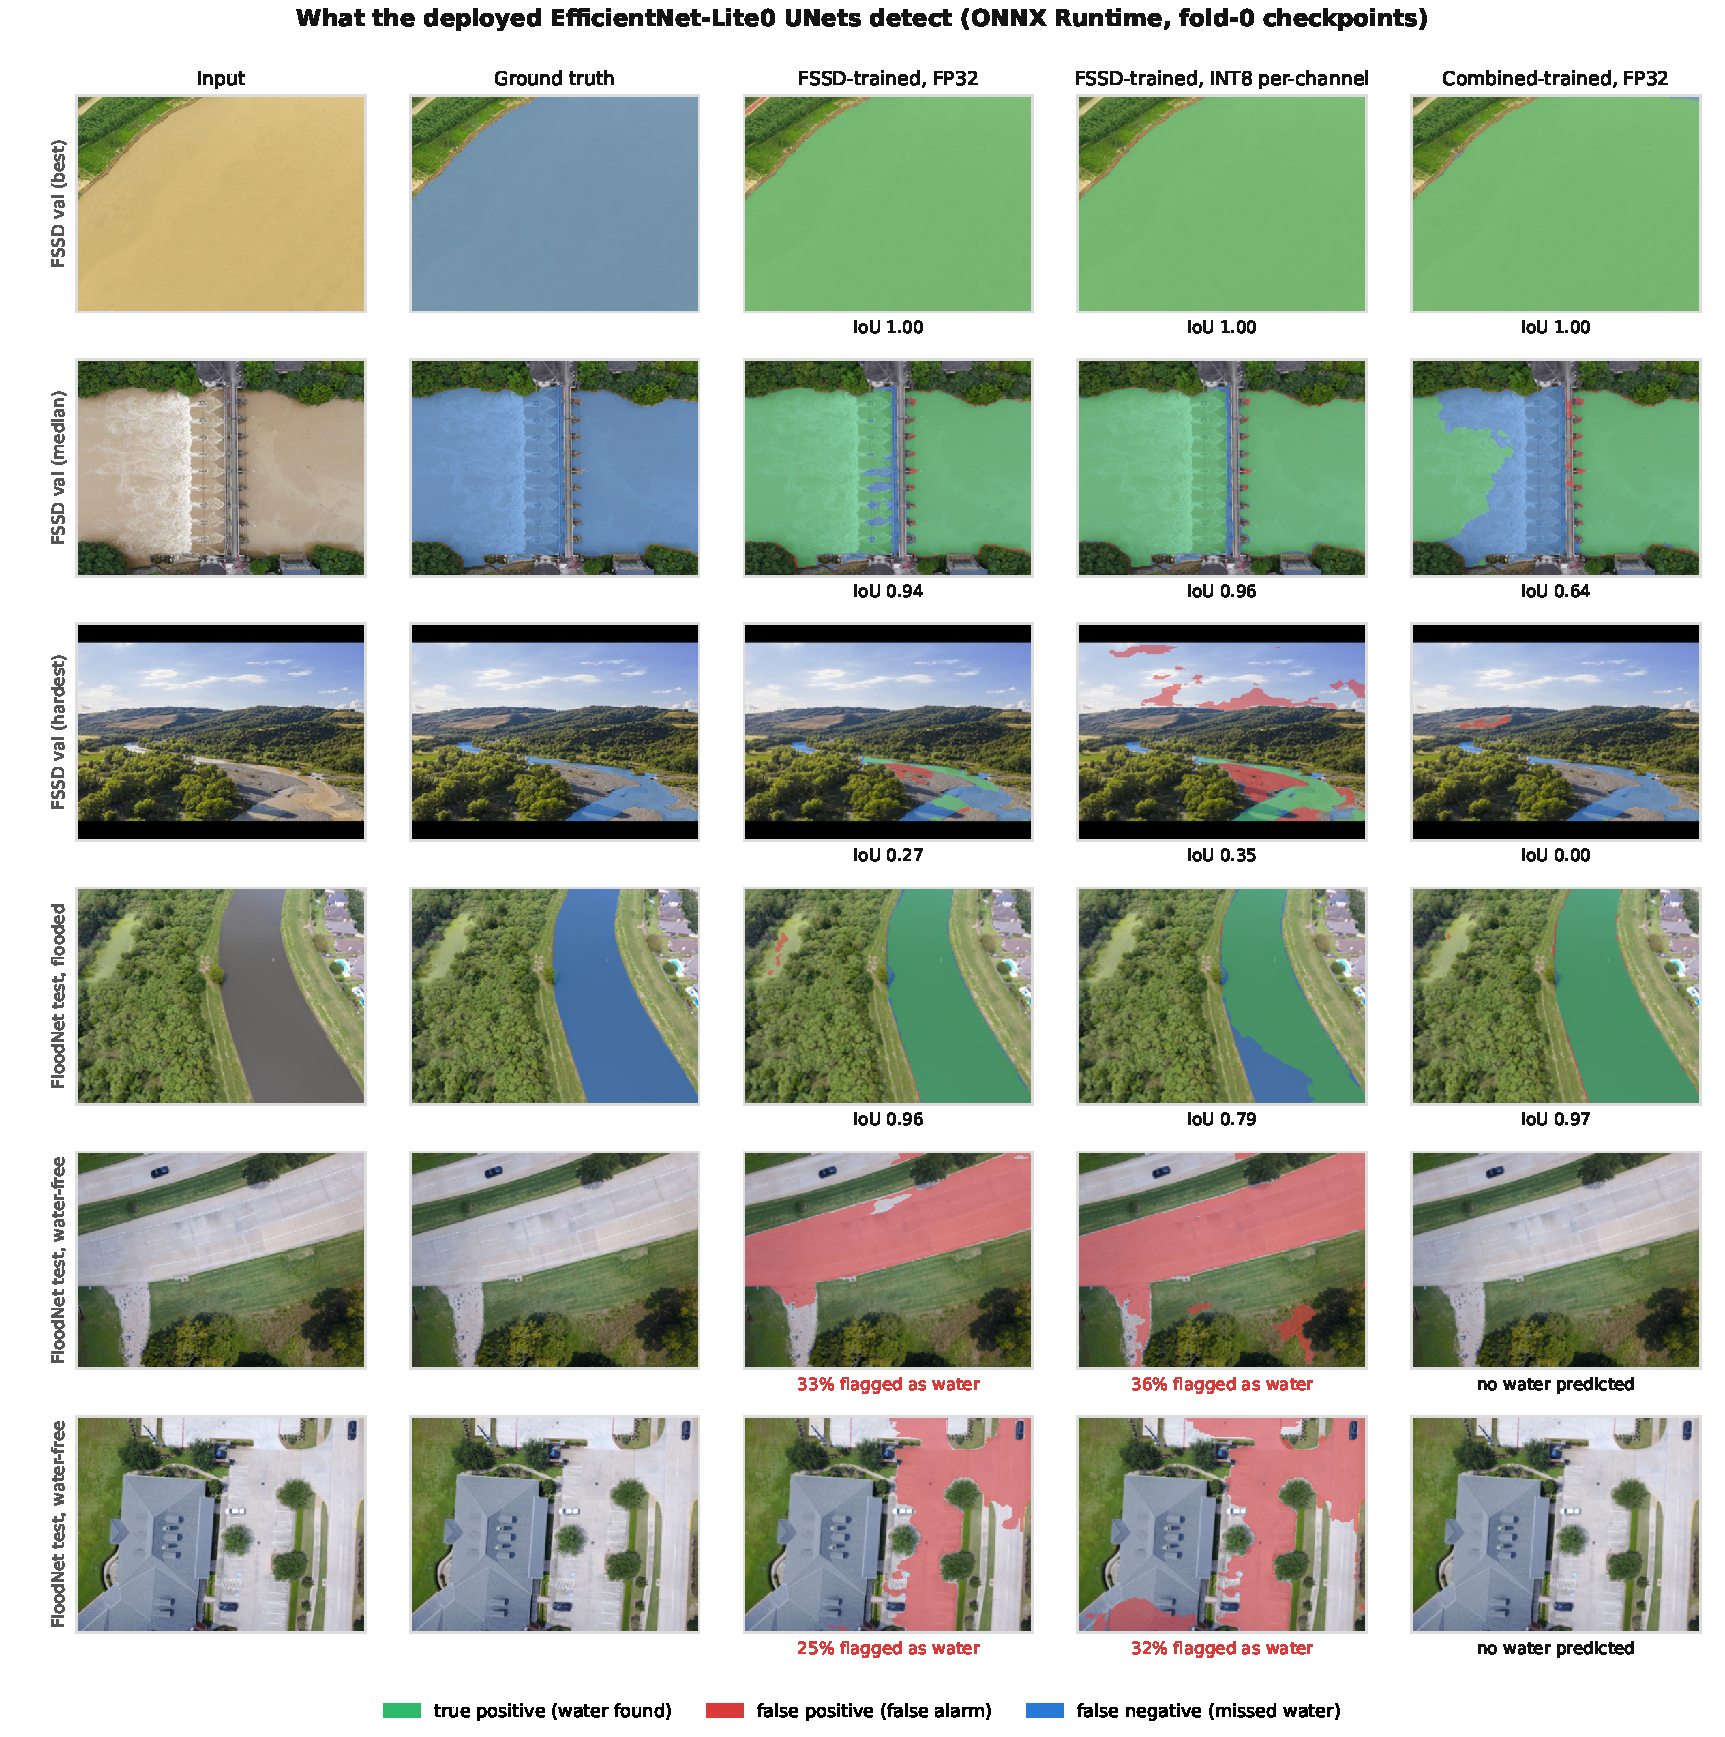
\includegraphics[width=0.9\linewidth]{figures/F7_detections.pdf}
\caption{\textbf{What the deployed EfficientNet-Lite0 UNets detect.} Rows: the best, median and hardest fold-0 FSSD validation images (ranked by FP32 IoU), a flooded FloodNet test scene, and two water-free FloodNet test scenes. Columns: input, ground truth (blue), and the overlays of three deployed models run through ONNX Runtime from their fold-0 checkpoints: FSSD-trained FP32, FSSD-trained INT8 (per-channel recipe) and combined-corpus-trained FP32. Green marks water found, red a false alarm, blue missed water. The number under each overlay is the IoU, or on the water-free scenes the share of pixels flagged as water.}
\label{fig:f7-detections}
\end{figure*}

\subsection{Out-of-distribution generalisation (Sen1Floods11)}
\label{sec:results-ood}

To test whether the FSSD-trained configurations transfer beyond their training distribution, we evaluate every model, with no fine-tuning, on 250 hand-labelled RGB chips from Sen1Floods11~\cite{bonafilia2020sen1floods11}, a Sentinel-2 optical flood benchmark whose top-down satellite viewpoint and sensor characteristics differ sharply from FSSD's close-range aerial, oblique, and ground photographs. Table~\ref{tab:t6-ood} reports the result, averaged over the three folds' checkpoints.

% =====================================================================
%  Table T6 -- Zero-shot Out-of-Distribution Transfer (Sen1Floods11)
%  Source of truth: code/runs/3fold/ood_results.json (aggregate over folds 0-2)
%  In-distribution FSSD IoU: code/runs/3fold/summary.json
% =====================================================================
\begin{table*}[ht]
\centering
\caption{\textbf{Zero-shot out-of-distribution transfer to Sen1Floods11.} FSSD-trained models (no fine-tuning) evaluated on 250 hand-labelled Sentinel-2 RGB chips; mean $\pm$ std over the three folds' checkpoints. In-distribution FSSD IoU (Table~\ref{tab:t2-segmentation}) is shown for reference. Metrics are computed per batch of 8 chips and averaged over batches (as in Tables~\ref{tab:t2-segmentation}--\ref{tab:t4-quant}), so the averaged F1 need not lie between the averaged precision and recall. Every model collapses to IoU $\approx 0.16$, a domain-shift effect that is uniform across teacher, baseline, and students.}
\label{tab:t6-ood}
\small
\setlength{\tabcolsep}{5pt}
\begin{adjustbox}{max width=\textwidth}
\begin{tabular}{lccccc}
\toprule
\textbf{Model} & \textbf{FSSD IoU} & \textbf{OOD IoU} & \textbf{OOD F1} & \textbf{OOD Prec} & \textbf{OOD Rec} \\
               & \textbf{(in-dist.)} & \multicolumn{4}{c}{\textbf{Sen1Floods11 (zero-shot)}} \\
\midrule
Teacher (UNet$+$EffB0)      & 0.9257 & 0.160 $\pm$ 0.007 & 0.246 $\pm$ 0.011 & 0.295 $\pm$ 0.022 & 0.271 $\pm$ 0.017 \\
MobileNetV2 baseline        & 0.9257 & 0.164 $\pm$ 0.005 & 0.248 $\pm$ 0.011 & 0.385 $\pm$ 0.019 & 0.230 $\pm$ 0.024 \\
MobileNetV3-S / none        & 0.9269 & 0.173 $\pm$ 0.006 & 0.269 $\pm$ 0.007 & 0.288 $\pm$ 0.011 & 0.317 $\pm$ 0.012 \\
EfficientNet-Lite0 / none   & 0.9277 & 0.155 $\pm$ 0.013 & 0.241 $\pm$ 0.016 & 0.333 $\pm$ 0.011 & 0.238 $\pm$ 0.025 \\
MobileViT-XXS / none        & 0.9367 & 0.169 $\pm$ 0.009 & 0.265 $\pm$ 0.008 & 0.242 $\pm$ 0.029 & 0.402 $\pm$ 0.036 \\
\bottomrule
\end{tabular}
\end{adjustbox}
\end{table*}


The transfer is poor across the board: every model collapses from IoU $\approx 0.93$ in-distribution to IoU $\approx 0.16$ on Sen1Floods11, a near-total loss of flood-pixel overlap. Two points matter for the deployment story. First, the collapse is essentially uniform across the teacher (0.160), the MobileNetV2 baseline (0.164), and the three lightweight students (0.155--0.173): it is a domain-shift effect, not a compression or capacity artefact. The recommended EfficientNet-Lite0 ($0.155 \pm 0.013$) is within one cross-fold standard deviation of the teacher ($0.160 \pm 0.007$) on the OOD set, so the OOD collapse does not single out the deployable student relative to the teacher; the two students that edge above the teacher (MobileNetV3-Small, 0.173; MobileViT-XXS, 0.169) do so within the same cross-fold noise. Second, in absolute terms IoU $\approx 0.16$ is not operationally useful: an FSSD-trained close-range-RGB model is \emph{not} a drop-in flood mapper for Sentinel-2 satellite optical imagery, and cross-sensor deployment requires domain adaptation or retraining on in-sensor data. The precision/recall split also mirrors the operational error asymmetry (Section~\ref{sec:discussion-asymmetry}): MobileViT-XXS reaches the highest OOD recall ($0.40$) at the cost of precision (it over-predicts flood, the safer direction for event-time mapping; Section~\ref{sec:discussion-asymmetry}), whereas the MobileNetV2 baseline is the most precision-favouring ($0.385$ precision, $0.230$ recall).

\subsection{Within-regime zero-shot generalisation and quantization under shift}
\label{sec:results-zeroshot}

The Sen1Floods11 result bounds the recommendations across \emph{sensors}; it leaves open how the models behave on unseen imagery from the regime they were built for: close-range RGB flood photography. Table~\ref{tab:t9-zeroshot} therefore evaluates the FSSD-trained models, without any fine-tuning, on two within-regime external sets with verified zero image overlap against FSSD (Section~\ref{sec:methods-data}): AIFloodSense (94 ground-level flood photographs) and the held-out FloodNet test split (424 UAV images, 215 of which contain no water). Each configuration is evaluated with all three folds' checkpoints; we report mean $\pm$ cross-fold standard deviation. Three results follow.

% =====================================================================
%  Table T9 -- Zero-shot generalization (FSSD-trained, no fine-tuning)
%  Source of truth: code/runs/3fold/zero_shot_3fold.json
%  (per-fold detail: zero_shot_fold{0,1,2}.json; aggregate_zero_shot.py)
% =====================================================================
\begin{table*}[ht]
\centering
\caption{\textbf{Zero-shot generalization of FSSD-trained models} (no fine-tuning; mean $\pm$ std across the three folds' checkpoints) on AIFloodSense (94 images, all flood-containing) and the held-out FloodNet test split (424 images, 215 of them water-free). Per-image macro metrics (Section~\ref{sec:setup-metrics}): IoU over all images, flood-only IoU over flood-containing images, and false-alarm rate (FAR) over water-free images. FSSD contains no water-free images, and every FP32 model false-alarms on 72--100\% of water-free FloodNet scenes (70\% for the distilled EfficientNet-Lite0 of Table~\ref{tab:t10-combined}; hence the 70--100\% quoted for all FSSD-trained models). INT8 rows are the no-KD students' ONNX exports under the per-tensor recipe of Table~\ref{tab:t4-quant} (PT) and the per-channel recipe of Table~\ref{tab:t12-ptq-mechanism} (PC). Under PT, degradation exceeds its in-domain counterpart, and MobileNetV3-Small's seemingly moderate overall FloodNet IoU is an artifact of near-constant background prediction (flood-only IoU 0.08); under PC, MobileNetV3-Small and EfficientNet-Lite0 recover to within 0.07 of FP32 on every metric, while MobileViT-XXS still loses 0.18--0.20.}
\label{tab:t9-zeroshot}
\small
\setlength{\tabcolsep}{4pt}
\begin{adjustbox}{max width=\textwidth}
\begin{tabular}{llcccc}
\toprule
& & \textbf{AIFloodSense} & \multicolumn{3}{c}{\textbf{FloodNet test}} \\
\cmidrule(lr){4-6}
\textbf{Model} & \textbf{Prec.} & \textbf{IoU} & \textbf{IoU (all)} & \textbf{IoU (flood)} & \textbf{FAR} \\
\midrule
Teacher (UNet$+$EffB0)  & FP32 & 0.706 $\pm$ 0.004 & 0.288 $\pm$ 0.014 & 0.509 $\pm$ 0.010 & 0.927 $\pm$ 0.018 \\
MobileNetV2 baseline    & FP32 & 0.690 $\pm$ 0.014 & 0.378 $\pm$ 0.015 & 0.475 $\pm$ 0.020 & 0.716 $\pm$ 0.040 \\
MobileNetV3-Small       & FP32 & 0.698 $\pm$ 0.008 & 0.285 $\pm$ 0.005 & 0.506 $\pm$ 0.012 & 0.929 $\pm$ 0.021 \\
EfficientNet-Lite0      & FP32 & 0.702 $\pm$ 0.006 & 0.388 $\pm$ 0.025 & 0.507 $\pm$ 0.021 & 0.727 $\pm$ 0.032 \\
MobileViT-XXS           & FP32 & 0.723 $\pm$ 0.006 & 0.253 $\pm$ 0.004 & 0.512 $\pm$ 0.007 & 1.000 $\pm$ 0.000 \\
\midrule
MobileNetV3-Small       & INT8 PT & 0.192 $\pm$ 0.164 & 0.355 $\pm$ 0.140 & 0.077 $\pm$ 0.073 & 0.375 $\pm$ 0.346 \\
EfficientNet-Lite0      & INT8 PT & 0.649 $\pm$ 0.028 & 0.258 $\pm$ 0.011 & 0.453 $\pm$ 0.032 & 0.932 $\pm$ 0.012 \\
MobileViT-XXS           & INT8 PT & 0.337 $\pm$ 0.078 & 0.092 $\pm$ 0.019 & 0.172 $\pm$ 0.049 & 0.986 $\pm$ 0.011 \\
\midrule
MobileNetV3-Small       & INT8 PC & 0.634 $\pm$ 0.023 & 0.248 $\pm$ 0.010 & 0.431 $\pm$ 0.010 & 0.930 $\pm$ 0.010 \\
EfficientNet-Lite0      & INT8 PC & 0.703 $\pm$ 0.002 & 0.283 $\pm$ 0.009 & 0.456 $\pm$ 0.026 & 0.885 $\pm$ 0.008 \\
MobileViT-XXS           & INT8 PC & 0.527 $\pm$ 0.036 & 0.164 $\pm$ 0.005 & 0.333 $\pm$ 0.011 & 1.000 $\pm$ 0.000 \\
\bottomrule
\end{tabular}
\end{adjustbox}
\end{table*}


\emph{First, FP32 students transfer as well as the teacher.} On AIFloodSense every FP32 model lands within 0.69--0.72 IoU with cross-fold standard deviations below 0.015; the best transfer is MobileViT-XXS ($0.723 \pm 0.006$), and the teacher holds no advantage ($0.706 \pm 0.004$). Combined KD transfers slightly \emph{worse} than no-KD on all three architectures ($-0.005$ to $-0.015$ IoU), extending the negative distillation result of Section~\ref{sec:results-kd} beyond the training distribution. On FloodNet's flood-containing images, all FP32 models cluster at 0.47--0.51 flood-IoU, a uniform $\sim$0.42-point drop from in-domain performance that reflects the viewpoint and resolution gap of high-altitude UAV imagery rather than any architecture-specific failure.

\emph{Second, FSSD-trained models cannot say ``no flood''.} Every FP32 model, teacher included, predicts water on 72--100\% of the 215 water-free FloodNet scenes (Table~\ref{tab:t9-zeroshot}, FAR column; MobileViT false-alarms on all of them in every fold). The cause is structural: FSSD contains flood imagery only, so the decision ``this scene contains no water'' is never supervised. For the monitoring use-cases that motivate edge deployment (continuous observation of scenes that are dry most of the time), this failure mode is disqualifying independently of segmentation quality, it is invisible to every FSSD-internal metric in Tables~\ref{tab:t2-segmentation}--\ref{tab:t4-quant}, and in unattended use it is the costly error (Section~\ref{sec:discussion-asymmetry}). Retraining on negative-image-bearing data (Section~\ref{sec:methods-data}) is the direct remedy; Section~\ref{sec:results-combined} tests it.

\emph{Third, INT8 degradation grows with distribution shift, and the per-tensor recipe is again most of the cause.} Under the per-tensor recipe, EfficientNet-Lite0-INT8 loses 0.043 IoU in-domain (Table~\ref{tab:t4-quant}) but 0.053 on AIFloodSense ($0.702 \rightarrow 0.649$) and 0.054 flood-IoU on FloodNet ($0.507 \rightarrow 0.453$), while its false-alarm rate jumps from 0.727 to 0.932: the quantized model fails the water-free scenes that its FP32 parent still partially rejects. The fragile architectures collapse outright: MobileNetV3-Small-INT8 drops to $0.192 \pm 0.164$ IoU on AIFloodSense and $0.077 \pm 0.073$ flood-IoU on FloodNet (its seemingly moderate overall FloodNet score ($0.355$) comes from predicting almost nothing, which is rewarded on the 215 water-free images), and MobileViT-XXS-INT8 loses more than half its FP32 transfer ($0.723 \rightarrow 0.337$). Re-quantizing the same checkpoints with per-channel weight scales (Section~\ref{sec:results-quant}) removes most of this. EfficientNet-Lite0 then matches its FP32 parent on AIFloodSense ($0.703 \pm 0.002$) and on FloodNet flood-IoU ($0.456 \pm 0.026$), and its false-alarm rate rises by 0.16 (to 0.885) instead of 0.21. MobileNetV3-Small recovers to $0.634 \pm 0.023$ on AIFloodSense and $0.431 \pm 0.010$ flood-IoU, and its FloodNet behaviour becomes that of its FP32 parent (FAR 0.930, overall IoU 0.248): false alarms on nearly every dry scene, but no empty predictions. MobileViT-XXS improves ($0.337 \rightarrow 0.527$ on AIFloodSense) but still loses 0.18--0.20 IoU on both sets, in line with its in-domain residual loss. Two points survive the recipe change. The per-channel losses of the two convolutional students on FloodNet (0.05--0.08 flood-IoU) are two to three times their in-domain losses, and INT8 raises the false-alarm rate of the one model that partially rejected dry scenes. PTQ calibrated on 80 in-domain images therefore degrades further under the distribution shift that defines real deployments, most visibly in false-alarm behaviour, and the recipe matters more under shift than in-domain validation suggests; we flag this as a practitioner trap that in-domain PTQ validation does not reveal, and note that it also illustrates why mixed test sets must be reported with split metrics rather than a single macro IoU.

\subsection{Retraining on data with water-free images}
\label{sec:results-combined}

Section~\ref{sec:results-zeroshot} attributes the false-alarm failure to FSSD's lack of water-free images. To test that attribution, and to ask whether the negative-KD result survives on a less saturated benchmark, we retrain the teacher and the three students under no-KD and combined KD on the combined corpus of Section~\ref{sec:methods-data}. Each fold trains on 2{,}057 images: 1{,}825 FloodNet train$+$val images (855 of them water-free) and the 232 Kaggle Flood Area Segmentation images outside the held-out fold. Model selection uses the held-out Kaggle fold (54--55 images after the duplicate filter, all flood-containing), and a source-balanced sampler draws each source equally often in expectation, because FloodNet outnumbers the Kaggle images about 8:1 and carries far less water per image. Everything else follows Section~\ref{sec:setup-impl}, except that students also use batch size 8. The FloodNet test split and AIFloodSense remain untouched by training and model selection, so the two regimes are compared on identical held-out images (Table~\ref{tab:t10-combined}). To fit the free-tier budget this experiment runs the reduced grid only: no response- or feature-only KD, no MobileNetV2 baseline, and no latency re-measurement (latency is a property of the architecture, not the weights).

% =====================================================================
%  Table T10 -- Combined-dataset retraining (D2) vs FSSD-trained zero-shot
%  Source of truth (combined-trained): code/runs/combined/summary.json
%    (per-fold detail: results_fold{0,1,2}.json; aggregate_combined.py)
%  Source of truth (FSSD-trained):     code/runs/3fold/zero_shot_3fold.json
%    (same rows as Table T9; std there)
% =====================================================================
\begin{table*}[ht]
\centering
\caption{\textbf{Retraining on negative-image-bearing data removes the false-alarm failure.} Left: FSSD-trained models evaluated zero-shot (means of Table~\ref{tab:t9-zeroshot}; standard deviations there). Right: the same configurations retrained on the combined corpus (Kaggle Flood Area Segmentation $+$ FloodNet train$+$val, 2{,}057 images of which 855 are water-free; Section~\ref{sec:results-combined}), mean $\pm$ std over three folds. FloodNet test (424 images, 215 water-free) and AIFloodSense are never used for training or model selection in either regime; AIFloodSense has 94 images on the left and 93 on the right, after the corpus's duplicate filter removes one copy. Per-image macro metrics as in Table~\ref{tab:t9-zeroshot}; FAR is the fraction of water-free scenes with any predicted water (lower is better). All models FP32.}
\label{tab:t10-combined}
\small
\setlength{\tabcolsep}{2pt}
\begin{adjustbox}{max width=\textwidth}
\begin{tabular}{llcccc@{\hskip 6pt}cccc}
\toprule
& & \multicolumn{4}{c}{\textbf{FSSD-trained (zero-shot)}} & \multicolumn{4}{c}{\textbf{Combined-trained}} \\
\cmidrule(lr){3-6}\cmidrule(lr){7-10}
& & \textbf{AIFS} & \multicolumn{3}{c}{\textbf{FloodNet test}} & \textbf{AIFS} & \multicolumn{3}{c}{\textbf{FloodNet test}} \\
\cmidrule(lr){4-6}\cmidrule(lr){8-10}
\textbf{Model} & \textbf{KD} & \textbf{IoU} & \textbf{IoU (all)} & \textbf{IoU (flood)} & \textbf{FAR} & \textbf{IoU} & \textbf{IoU (all)} & \textbf{IoU (flood)} & \textbf{FAR} \\
\midrule
Teacher (UNet$+$EffB0) & --   & 0.706 & 0.288 & 0.509 & 0.927 & 0.731 $\pm$ 0.011 & 0.783 $\pm$ 0.082 & 0.781 $\pm$ 0.003 & 0.216 $\pm$ 0.165 \\
\midrule
MobileNetV3-Small      & none & 0.698 & 0.285 & 0.506 & 0.929 & 0.713 $\pm$ 0.008 & 0.860 $\pm$ 0.023 & 0.754 $\pm$ 0.011 & 0.037 $\pm$ 0.036 \\
                       & comb & 0.693 & 0.280 & 0.497 & 0.930 & 0.725 $\pm$ 0.012 & 0.848 $\pm$ 0.018 & 0.780 $\pm$ 0.014 & 0.085 $\pm$ 0.047 \\
EfficientNet-Lite0     & none & 0.702 & 0.388 & 0.507 & 0.727 & 0.731 $\pm$ 0.005 & 0.854 $\pm$ 0.006 & 0.736 $\pm$ 0.015 & 0.031 $\pm$ 0.010 \\
                       & comb & 0.690 & 0.399 & 0.503 & 0.702 & 0.739 $\pm$ 0.008 & 0.844 $\pm$ 0.031 & 0.779 $\pm$ 0.015 & 0.093 $\pm$ 0.060 \\
MobileViT-XXS          & none & 0.723 & 0.253 & 0.512 & 1.000 & 0.738 $\pm$ 0.012 & 0.831 $\pm$ 0.017 & 0.695 $\pm$ 0.027 & 0.037 $\pm$ 0.009 \\
                       & comb & 0.708 & 0.262 & 0.507 & 0.975 & 0.727 $\pm$ 0.006 & 0.854 $\pm$ 0.011 & 0.762 $\pm$ 0.018 & 0.057 $\pm$ 0.035 \\
\bottomrule
\end{tabular}
\end{adjustbox}
\end{table*}


\emph{First, the false-alarm failure disappears.} Combined-trained students false-alarm on 3--9\% of the 215 water-free FloodNet scenes (Table~\ref{tab:t10-combined}), against 70--100\% for the same configurations trained on FSSD. Flood-only IoU on FloodNet rises from 0.50--0.51 to 0.70--0.78, and macro IoU from 0.25--0.40 to 0.83--0.86. This confirms that the failure in Section~\ref{sec:results-zeroshot} was a training-data property, not an architectural one: none of the three lightweight backbones lacks the capacity to reject a dry scene once dry scenes are supervised. AIFloodSense, which neither regime trains on, improves by a smaller margin (0.69--0.72 $\rightarrow$ 0.71--0.74).

\emph{Second, the teacher is the least reliable rejector.} Teacher false-alarm rates vary by more than an order of magnitude across folds (0.279, 0.028, 0.340), while every no-KD student stays at or below 0.08 in every fold. The teacher still has the highest flood-only IoU (0.781), so its lower macro IoU (0.783 vs.\ 0.831--0.860 for the students) comes entirely from false alarms. A plausible cause is model selection: the validation fold contains no water-free image, so checkpoint selection rewards flood segmentation and is blind to rejection behaviour. We have not tested this explanation.

\emph{Third, distillation now helps segmentation but transmits the teacher's false alarms.} On this benchmark combined KD raises FloodNet flood-only IoU for every student in every fold (9 of 9 student--fold pairs). Pooling per-image differences over the 209 flood-containing test images (averaged over folds, 10{,}000 bootstrap replicates), the gain is $+0.026$ [95\% CI $+0.015$, $+0.038$] for MobileNetV3-Small, $+0.043$ [$+0.030$, $+0.057$] for EfficientNet-Lite0, and $+0.067$ [$+0.048$, $+0.087$] for MobileViT-XXS. The same distillation raises the false-alarm rate by $+0.048$ [$+0.028$, $+0.070$] and $+0.062$ [$+0.040$, $+0.084$] for the first two students; for MobileViT-XXS the increase ($+0.020$ [$-0.000$, $+0.042$]) is not significant. The extra false alarms are concentrated on the scenes where the teacher itself false-alarms. Over all water-free test images and folds, the teacher false-alarms in 139 of 645 image--fold cases. On those, distilled students false-alarm 23--33\% of the time against 10--14\% for their no-KD counterparts; on the remaining 506 the rates are 0.6--3.2\% with or without distillation. The no-KD rate is itself elevated on the teacher's false-alarm scenes, so some of these images are intrinsically hard. To test whether the KD effect is specific to them, we compute a difference-in-differences: the KD-induced change in false-alarm rate on teacher-false-alarm cases minus the change on teacher-correct cases, with a bootstrap that resamples images (keeping each image's three fold copies together; 10{,}000 replicates; \texttt{scripts/stats\_combined.py}). It is $+0.186$ [$+0.114$, $+0.263$] for MobileNetV3-Small, $+0.169$ [$+0.093$, $+0.246$] for EfficientNet-Lite0, and $+0.139$ [$+0.069$, $+0.214$] for MobileViT-XXS. Distillation therefore adds false alarms mainly where the teacher makes them, although for EfficientNet-Lite0 it also adds a small number elsewhere ($+0.026$ on teacher-correct cases). This pattern is consistent with the student imitating the teacher's outputs on those scenes; our design does not separate the response and feature terms, so we cannot say which carries the effect. On AIFloodSense the effect of distillation is mixed ($+0.012$, $+0.008$, $-0.011$ IoU).

\emph{Fourth, the per-tensor quantization split survives retraining, per-channel scales again repair the convolutional students, and INT8 costs more than in-domain validation shows.} We apply both the per-tensor recipe of Table~\ref{tab:t4-quant} and the per-channel recipe of Table~\ref{tab:t12-ptq-mechanism} to all eighteen combined-trained checkpoints (Table~\ref{tab:t11-combined-int8}). Under per-tensor scales EfficientNet-Lite0 again quantizes stably on its validation fold ($0.781 \rightarrow 0.751$), while MobileNetV3-Small and MobileViT-XXS collapse again ($0.778 \rightarrow 0.458$ and $0.780 \rightarrow 0.193$, with cross-fold standard deviations of 0.18--0.23), so the split is not an artefact of FSSD. Per-channel scales recover MobileNetV3-Small on every split (validation $0.739 \pm 0.061$, FloodNet flood-IoU $0.649 \pm 0.057$, FAR $0.081 \pm 0.073$, AIFloodSense $0.687 \pm 0.021$), as Section~\ref{sec:results-quant} predicts, and improve EfficientNet-Lite0 by 0.01--0.04 on every accuracy metric. They do not recover MobileViT-XXS: its per-fold validation IoU under per-channel scales is $0.449/0.032/0.133$ without KD and $0.566/0.040/0.040$ with KD, an outright collapse in two of three folds and deeper than the 0.22--0.33 loss the same recipe produces on FSSD. Two further results matter for deployment. First, even the stable backbone loses far more on the FloodNet test split than on its validation fold: no-KD EfficientNet-Lite0 drops from 0.736 to $0.589 \pm 0.086$ flood-only IoU under per-tensor and to $0.625 \pm 0.074$ under per-channel scales, about five times its validation loss under either recipe, against 0.02--0.04 IoU on AIFloodSense; validating INT8 on a small in-domain fold understates its cost. Second, quantization keeps the no-KD student's false alarms low ($0.031 \rightarrow 0.048$ and $0.051$) but amplifies the distilled student's ($0.093 \rightarrow 0.316 \pm 0.250$ and $0.341 \pm 0.273$) under both recipes, and per-channel MobileNetV3-Small shows the same pattern ($0.037 \rightarrow 0.081$ without KD, $0.085 \rightarrow 0.184$ with). The collapsed per-tensor backbones fail in both directions, predicting water nearly everywhere (MobileNetV3-Small with KD, FAR 0.97) or almost nowhere (MobileViT-XXS without KD, flood-only IoU 0.12).

% =====================================================================
%  Table T11 -- INT8 PTQ of the combined-trained students (D3 + D3b)
%  Source of truth: code/runs/combined/quantized.json     (per-tensor;
%                     scripts/quantize_combined.py, ONNX Runtime 1.22.1)
%                   code/runs/combined/quantized_pc.json  (per-channel;
%                     scripts/quantize_combined_pc.py, ONNX Runtime 1.22.1)
%  std = sample std (ddof=1) over the three folds, as in quantized.json.
% =====================================================================
\begin{table*}[ht]
\centering
\caption{\textbf{INT8 post-training quantization of the combined-trained students} under the per-tensor recipe of Table~\ref{tab:t4-quant} (PT) and the per-channel-weight recipe of Table~\ref{tab:t12-ptq-mechanism} (PC); both use static QDQ with Percentile-99.999\% calibration on 80 training images of the fold. FP32 values are the ONNX exports of the Table~\ref{tab:t10-combined} checkpoints (means over three folds); INT8 values are mean $\pm$ std over the three folds. Val is the held-out Kaggle fold (54--55 flood images); FloodNet test and AIFloodSense as in Table~\ref{tab:t10-combined}. Per-channel scales recover MobileNetV3-Small on every split but leave MobileViT-XXS collapsed (per-fold val IoU $0.449/0.032/0.133$ without KD). A low INT8 FAR on a collapsed model reflects near-empty predictions, not good rejection; read it with the flood-only IoU.}
\label{tab:t11-combined-int8}
\small
\setlength{\tabcolsep}{2.2pt}
\begin{adjustbox}{max width=\textwidth}
\begin{tabular}{llccc@{\hskip 6pt}ccc@{\hskip 6pt}ccc@{\hskip 6pt}ccc}
\toprule
& & \multicolumn{3}{c}{\textbf{Val IoU}} & \multicolumn{3}{c}{\textbf{FloodNet IoU (flood)}} & \multicolumn{3}{c}{\textbf{FloodNet FAR}} & \multicolumn{3}{c}{\textbf{AIFS IoU}} \\
\cmidrule(lr){3-5}\cmidrule(lr){6-8}\cmidrule(lr){9-11}\cmidrule(lr){12-14}
\textbf{Model} & \textbf{KD} & FP32 & INT8 PT & INT8 PC & FP32 & INT8 PT & INT8 PC & FP32 & INT8 PT & INT8 PC & FP32 & INT8 PT & INT8 PC \\
\midrule
MobileNetV3-Small  & none & 0.778 & 0.458 $\pm$ 0.176 & 0.739 $\pm$ 0.061 & 0.754 & 0.215 $\pm$ 0.176 & 0.649 $\pm$ 0.057 & 0.037 & 0.584 $\pm$ 0.512 & 0.081 $\pm$ 0.073 & 0.713 & 0.445 $\pm$ 0.159 & 0.687 $\pm$ 0.021 \\
                   & comb & 0.783 & 0.477 $\pm$ 0.231 & 0.759 $\pm$ 0.030 & 0.780 & 0.324 $\pm$ 0.119 & 0.698 $\pm$ 0.082 & 0.085 & 0.966 $\pm$ 0.059 & 0.184 $\pm$ 0.140 & 0.725 & 0.491 $\pm$ 0.179 & 0.704 $\pm$ 0.017 \\
\textbf{EfficientNet-Lite0} & none & 0.781 & 0.751 $\pm$ 0.032 & \textbf{0.759 $\pm$ 0.026} & 0.736 & 0.589 $\pm$ 0.086 & \textbf{0.625 $\pm$ 0.074} & 0.031 & 0.048 $\pm$ 0.047 & \textbf{0.051 $\pm$ 0.057} & 0.731 & 0.689 $\pm$ 0.024 & \textbf{0.715 $\pm$ 0.007} \\
                   & comb & 0.784 & 0.753 $\pm$ 0.033 & 0.777 $\pm$ 0.028 & 0.779 & 0.632 $\pm$ 0.018 & 0.681 $\pm$ 0.028 & 0.093 & 0.316 $\pm$ 0.250 & 0.341 $\pm$ 0.273 & 0.739 & 0.693 $\pm$ 0.027 & 0.725 $\pm$ 0.009 \\
MobileViT-XXS      & none & 0.780 & 0.193 $\pm$ 0.204 & 0.205 $\pm$ 0.218 & 0.695 & 0.123 $\pm$ 0.176 & 0.143 $\pm$ 0.103 & 0.037 & 0.090 $\pm$ 0.156 & 0.017 $\pm$ 0.030 & 0.738 & 0.160 $\pm$ 0.195 & 0.217 $\pm$ 0.243 \\
                   & comb & 0.801 & 0.197 $\pm$ 0.200 & 0.215 $\pm$ 0.304 & 0.762 & 0.126 $\pm$ 0.159 & 0.169 $\pm$ 0.115 & 0.057 & 0.499 $\pm$ 0.500 & 0.087 $\pm$ 0.123 & 0.727 & 0.150 $\pm$ 0.140 & 0.186 $\pm$ 0.281 \\
\bottomrule
\end{tabular}
\end{adjustbox}
\end{table*}


The negative-KD finding of Section~\ref{sec:results-kd} is therefore specific to the saturated FSSD regime. When the teacher has headroom over the students on the positive class (teacher flood-only IoU 0.781 vs.\ 0.695--0.754 without KD), distillation recovers most of that gap, but it imports the teacher's rejection errors along with it. For unattended monitoring, where false alarms carry the operational cost (Section~\ref{sec:discussion-asymmetry}), the no-KD students are the safer choice, and they keep their false-alarm rates low after INT8 conversion (EfficientNet-Lite0 under either recipe, MobileNetV3-Small with per-channel scales), whereas the distilled students' rates double or triple. For event-time mapping, where missed flood pixels matter more, combined KD is worth its cost only if the teacher's own false-alarm rate is first verified on water-free data.

% =====================================================================
%  Section 6 -- Discussion
% =====================================================================

\section{Discussion}
\label{sec:discussion}

\subsection{What the negative KD result means}
\label{sec:discussion-negative-kd}

On FSSD, knowledge distillation does not help when the student is an ImageNet-pretrained lightweight UNet. We frame this as a \emph{negative result} rather than a \emph{null result} because the comparison is not ``we did not find a positive effect'' but rather ``the best student (MobileViT-XXS, no-KD) \emph{exceeds} the teacher (UNet$+$EfficientNet-B0)''. Distillation on this benchmark is at best redundant and at worst counter-productive: combined KD on MobileViT-XXS produced $-0.005$ IoU vs.~the same architecture trained without it.

We interpret this mechanistically. The classical motivation for KD, Hinton's \emph{dark knowledge} argument~\cite{hinton2015distilling} and subsequent feature-map alignment work~\cite{romero2015fitnets,liu2019structured,wang2020intra,he2021channel} assumes that the student has insufficient capacity or pretraining to recover the teacher's behaviour from labelled data alone, so the teacher's soft probabilities and intermediate features provide a richer supervision signal than the binary mask. On FSSD, that assumption is violated in two directions: (i)~the benchmark has only 663 images and saturates at IoU $\approx 0.93$, so the labelled signal is already nearly sufficient; and (ii)~the student's ImageNet pretraining already supplies the visual priors (edge detectors, texture filters, semantic-region features) that a teacher trained on the same FSSD would have been transferring. The teacher's ``dark knowledge'' is therefore largely redundant with the student's pretraining, and the response-based KL term reduces to a noise-injection regulariser. The feature-MSE term comes closest to the no-KD baseline (MobileViT-XXS: $-0.0011$ IoU, against $-0.0041$ for response-only and $-0.0049$ for combined KD; Table~\ref{tab:t3-kd-ablation}), plausibly because it carries at least \emph{some} signal beyond the labels, but it still does not beat the baseline.

This finding has two implications for the flood-segmentation literature:

\begin{enumerate}
\item \textbf{Benchmarks matter.} A KD recipe that wins on Cityscapes (19 classes, 5000 images, IoU $\approx 0.80$--$0.85$) does not transfer to FSSD (2 classes, 663 images, IoU $\approx 0.93$). Future KD work in this space should report headroom (teacher--best-pretrained-student gap) \emph{before} claiming distillation effects.
\item \textbf{Modern ImageNet pretraining is doing the work.} Current \texttt{timm}-pretrained lightweight backbones brings the no-KD baseline so high that compression strategies \emph{other than} distillation (quantization, pruning, architecture choice) dominate the deployment-relevant trade-offs. We recommend that authors investing in flood-segmentation compression budget their effort accordingly.
\end{enumerate}

The combined-corpus experiment (Section~\ref{sec:results-combined}) supports the headroom reading and adds a caveat. Where the teacher out-segments the no-KD students on flood pixels (0.781 vs.\ 0.695--0.754 flood-only IoU), combined KD closes most of the gap, with the gain significant for all three students. It also transmits the teacher's false alarms: distilled students fire on the teacher's false-alarm scenes 2.3--2.6 times as often as their no-KD counterparts, and the increase is specific to those scenes. A student trained to imitate the teacher imitates its errors too. A teacher should therefore be audited on the failure mode that matters for deployment, here false alarms on dry scenes, before it is used for distillation, not only on the headline IoU that selects it.

\subsection{Per-platform deployment recommendations}
\label{sec:discussion-deployment}

Based on the joint segmentation $\times$ latency $\times$ stability evidence (Sections~\ref{sec:results-kd}--\ref{sec:results-latency}), we make the following deployment recommendations:

\begin{itemize}
\item \textbf{Field-laptop / tablet inference (Apple Silicon class):} EfficientNet-Lite0 UNet INT8. 17\,ms p50 (\deployableMTwoFPS~FPS) at IoU 0.885, $3.83\times$ size reduction. Stable across folds ($\pm 0.015$) even under the per-tensor recipe. This is the configuration we ship in our public release.
\item \textbf{Field-laptop / desktop inference (x86 class):} FP32, not INT8. On the Ryzen host INT8 is $2.8$--$3.0\times$ slower than FP32 for every network (Table~\ref{tab:t13-host2}), so the fastest configurations are FP32 MobileNetV3-Small (15\,ms) and FP32 EfficientNet-Lite0 (17\,ms); INT8 is worth its $3.4$--$3.8\times$ smaller file only when download size, not speed, is the constraint. Any INT8 deployment should be timed on the target CPU before it is shipped.
\item \textbf{Browser citizen-science / web-portal inference:} MobileNetV3-Small UNet FP32 (133\,ms p50; 7.5\,FPS on the M2 host), or MobileViT-XXS UNet FP32 (149\,ms p50; 6.7\,FPS) for slightly higher accuracy. Under ONNX Runtime Web~$\geq 1.18$ the INT8 artifacts load and run $1.3$--$1.4\times$ faster than FP32 (Table~\ref{tab:t13-host2}); per-channel INT8 MobileNetV3-Small (IoU 0.904, 3.8\,MB) is then the fastest and smallest browser option.
\item \textbf{Maximum-accuracy off-line inference:} MobileViT-XXS UNet FP32 (28\,ms p50 on M2~Pro CPU; IoU 0.937). Recommended for human-in-the-loop annotation pipelines.
\end{itemize}

The case against deploying the teacher (UNet$+$EffB0) is weaker than a latency-only comparison suggests. On a common ONNX Runtime CPU backend the teacher runs at 37.6\,ms p50 (\teacherMTwoFPS~FPS) on the M2~Pro and 23.4\,ms on the Ryzen, only $1.1$--$1.9\times$ slower than the FP32 students, and with per-channel scales it INT8-quantizes to IoU $0.917 \pm 0.005$ at 6.3\,MB (Table~\ref{tab:t12-ptq-mechanism}), which is more accurate than any INT8 student. What remains of the case is latency on the hardware where INT8 pays: the recommended EfficientNet-Lite0 INT8 is $2.2\times$ faster than the FP32 teacher on the M2~Pro (17.3 vs 37.6\,ms) while recovering 95\% of its IoU, and we did not time the INT8 teacher on that host. Where INT8 does not pay (the x86 host), the FP32 students are $1.1$--$1.5\times$ faster than the teacher, and a practitioner who can afford 23\,ms per image loses nothing by deploying the teacher itself.

Table~\ref{tab:t7-decision} consolidates these recommendations into a decision matrix, pairing each operational scenario with the configuration we recommend and the metric that decides it.

All of these recommendations carry the zero-shot caveats of Sections~\ref{sec:results-ood} and~\ref{sec:results-zeroshot}: the artifacts are validated for in-domain, close-range RGB; FSSD-trained models false-alarm on the majority of water-free scenes and must be retrained on negative-image-bearing data before \emph{unattended} monitoring use (Section~\ref{sec:results-combined} shows that this retraining brings student false-alarm rates down to 3--9\%, and that no-KD students are the safer choice there); and INT8 artifacts in particular should be re-validated on in-deployment-domain imagery, since their degradation worsens under distribution shift in a way that in-domain calibration metrics do not predict. The INT8 recommendations above also assume a CPU on which INT8 is faster than FP32; Table~\ref{tab:t13-host2} shows one on which it is not.

% =====================================================================
%  Table T7 -- Deployment Decision Matrix
%  Source of truth: summary.json (FP32 IoU), quantized.json (INT8 IoU),
%  lat_m2.json / lat_wasm.json (latency), T1 (size), T6 (OOD).
%  Re-presentation of the Section 6.2 recommendations; no new experiments.
% =====================================================================
\begin{table*}[ht]
\centering
\caption{\textbf{Deployment decision matrix.} Recommended configuration per operational scenario, with the deciding metrics. All values are drawn from Tables~\ref{tab:t1-footprints}, \ref{tab:t2-segmentation}, \ref{tab:t4-quant}, \ref{tab:t5-latency}, \ref{tab:t6-ood}, and~\ref{tab:t10-combined}; this table re-presents the Section~\ref{sec:discussion-deployment} recommendations as an at-a-glance practitioner reference and introduces no new experiments. Latency is p50 on the platform relevant to each scenario (Apple~M2~Pro ORT-CPU, or browser WASM SIMD on the M2 host); Table~\ref{tab:t13-host2} gives the x86 counterparts.}
\label{tab:t7-decision}
\small
\setlength{\tabcolsep}{4pt}
\begin{adjustbox}{max width=\textwidth}
\begin{tabular}{p{2.9cm}lcccp{6.2cm}}
\toprule
\textbf{Deployment scenario} & \textbf{Recommended} & \textbf{IoU} & \textbf{Latency (p50)} & \textbf{Size (MB)} & \textbf{Rationale / caveat} \\
\midrule
Field laptop / tablet (Apple-Silicon CPU)
  & \textbf{EffLite0-UNet INT8} & 0.885 & 17\,ms (M2) & 5.2
  & Fastest operating point on Apple Silicon (INT8 $2\times$ faster than FP32); the only student stable under per-tensor INT8 ($\pm 0.015$). On the x86 host INT8 is $2.8\times$ \emph{slower}: use FP32 there (Table~\ref{tab:t13-host2}). FSSD-trained, it false-alarms on 93\% of dry scenes (Table~\ref{tab:t9-zeroshot}): analyst-in-the-loop use only. \\
\addlinespace
Browser / citizen-science web portal
  & MNV3-S-UNet FP32 & 0.927 & 133\,ms (WASM) & 13.8
  & Fastest under single-threaded WASM SIMD; MobileViT-XXS FP32 (149\,ms, IoU 0.937) if accuracy matters more. Under ORT-Web~1.22 INT8 runs $1.3$--$1.4\times$ faster (Table~\ref{tab:t13-host2}); per-channel INT8 MobileNetV3-Small (IoU 0.904, 3.8\,MB) is then the smallest option. \\
\addlinespace
Maximum-accuracy off-line / human-in-the-loop
  & MobileViT-XXS-UNet FP32 & 0.937 & 28\,ms (M2) & 12.0
  & Highest IoU of any configuration; FP32 only (its INT8 loses $\geq 0.22$ IoU under every full-quantization recipe we tested, Table~\ref{tab:t12-ptq-mechanism}). \\
\addlinespace
Unattended monitoring (mostly dry scenes)
  & EffLite0-UNet FP32, no KD & 0.736\textsuperscript{$\ddagger$} & 34\,ms (M2) & 19.8
  & Must be retrained with water-free images: FSSD-trained models false-alarm on 70--100\% of dry scenes, combined-trained Lite0 on 3\% (Table~\ref{tab:t10-combined}). Lite0 over MobileNetV3-S because its INT8 variant is stable under either recipe (per-channel: FAR 0.051, flood IoU 0.625), whereas MobileNetV3-S is usable in INT8 only with per-channel scales (Table~\ref{tab:t11-combined-int8}). Skip KD: it inherits the teacher's false alarms. \\
\addlinespace
Cross-sensor / satellite optical
  & \emph{retrain / domain-adapt} & 0.16\textsuperscript{$\dagger$} & -- & --
  & No FSSD-trained model transfers zero-shot (Table~\ref{tab:t6-ood}); requires domain adaptation or in-sensor training data. \\
\bottomrule
\end{tabular}
\end{adjustbox}
\\[3pt]
{\footnotesize \textsuperscript{$\dagger$}Zero-shot Sen1Floods11 IoU; all models $\approx 0.16$ (Section~\ref{sec:results-ood}). \textsuperscript{$\ddagger$}Flood-only IoU on the FloodNet test split after combined-corpus retraining (Section~\ref{sec:results-combined}); not comparable with the FSSD IoUs above.}
\end{table*}


\subsection{The PTQ practitioner trap is the default recipe, not the architecture}
\label{sec:discussion-ptq-trap}

The 0.45-IoU PTQ collapse on MobileNetV3-Small and MobileViT-XXS would not be predicted from the classification-quantization literature, which typically reports about one point of top-1 accuracy lost to INT8 PTQ on ResNet/MobileNet/EfficientNet families on ImageNet~\cite{krishnamoorthi2018quantizing,jacob2018quantization}. That literature, however, assumes per-channel weight quantization for depthwise-separable networks, and Krishnamoorthi~\cite{krishnamoorthi2018quantizing} already reports that per-tensor weights drive MobileNet-family models to near-zero accuracy. Our ablation (Section~\ref{sec:results-quant}) reproduces exactly this on segmentation: the fold-dependent collapse of MobileNetV3-Small ($0.772$, $0.0001$ and $0.657$ IoU across folds) and the $0.19$--$0.30$ IoU loss of the teacher both disappear once the weight quantizer is per-channel, and keeping the HardSwish layers in FP32 adds nothing. We had attributed these collapses to the HardSwish activation range, which we had measured and found to be $12$--$17\times$ wider than ReLU6's; the measurement was correct and the inference from it was not. Two features of the segmentation setting still make the per-tensor failure worse than in classification: the output is a per-pixel binary mask, so a biased post-sigmoid threshold shifts the whole segmentation, and the collapse is fold-dependent, so a single validation fold can pass an artifact that fails on the next.

MobileViT-XXS is the genuine architectural case, but not for the reason the transformer-quantization literature would suggest. Its attention and LayerNorm blocks, which that literature identifies as the fragile components~\cite{lin2022fqvit,li2023repqvit}, quantize at no measurable cost here; the loss sits in the two high-resolution MobileNetV2-style stages before the first transformer block, which per-channel scales do not fix. The loss is not a property of the FSSD weights either: the same per-channel recipe collapses the combined-trained MobileViT-XXS outright in two of three folds (Table~\ref{tab:t11-combined-int8}). Why these stages fail in MobileViT-XXS and not in MobileNetV3-Small or the teacher, whose early blocks are of the same type, is open; the differences we can point to are MobileViT-XXS's very narrow early channel widths (16--24) and its SiLU activations in those blocks, and distinguishing them needs per-layer activation statistics we have not collected.

The practical guidance has therefore changed. A practitioner who runs the default ONNX Runtime static-quantization recipe on a lightweight segmentation backbone and sees it collapse should first switch \texttt{per\_channel} on; for every convolutional network in this study that one setting turns a collapse into a 0.01--0.04 IoU loss, on both training corpora and under zero-shot transfer (Tables~\ref{tab:t9-zeroshot} and~\ref{tab:t11-combined-int8}). Only if the loss persists, as it does for MobileViT-XXS, is the architecture the problem, and the next steps are keeping the identified layers in FP32 or quantization-aware training. In either case the INT8 artifact should be validated on every fold and on out-of-domain imagery (Section~\ref{sec:results-zeroshot}), and timed on the target CPU, since INT8 is not faster everywhere (Section~\ref{sec:results-latency}).

\subsection{Qualitative failure modes}
\label{sec:discussion-failures}

Figure~\ref{fig:f3-qualitative} shows that both teacher and EfficientNet-Lite0-INT8 student share two persistent failure modes:
\begin{itemize}
\item \textbf{Bright-reflective-surface confusion:} wet asphalt, glare-on-roof, and large reflective puddles are misclassified as flood. This is a labelling-modality issue, not a model-capacity issue: RGB alone cannot disambiguate water from wet non-water surfaces.
\item \textbf{Vegetation-occluded edges:} when flooded water is partially overhung by trees or tall grass, both models under-segment the flood boundary. The 5-pixel margin at the boundary contributes disproportionately to the residual IoU gap.
\end{itemize}

Both failure modes argue for SAR or multispectral fusion rather than for a different RGB segmentation recipe. We discuss this in Section~\ref{sec:limitations}.

Table~\ref{tab:t8-taxonomy} organises the failure modes observed across the whole study (the two RGB-modality failures above, the cross-sensor distribution shift of Section~\ref{sec:results-ood}, and the INT8 PTQ failures of Section~\ref{sec:results-quant}) into a single taxonomy, noting for each its mechanism, error direction, the models affected, and the mitigation it implies. The categories are qualitative: we report the error direction (which matters for the operational cost asymmetry of Section~\ref{sec:discussion-asymmetry}) but do not claim per-class frequencies.

% =====================================================================
%  Table T8 -- Error Taxonomy
%  Qualitative synthesis of failure modes established in
%  Sections 5.3 (PTQ), 5.7 (OOD), 6.4 (qualitative failure modes).
%  No new experiments; per-class frequencies are NOT claimed.
% =====================================================================
\begin{table*}[ht]
\centering
\caption{\textbf{Error taxonomy for FSSD flood segmentation.} Four failure classes observed across this study, their mechanism, the direction of the resulting error (which direction costs more depends on the use: false negatives in event-time mapping, false positives in unattended monitoring, Section~\ref{sec:discussion-asymmetry}), the models affected, and the mitigation each implies. Categories are qualitative, synthesised from Sections~\ref{sec:results-quant}, \ref{sec:results-ood}, and~\ref{sec:discussion-failures}; we do not claim per-class frequencies.}
\label{tab:t8-taxonomy}
\small
\setlength{\tabcolsep}{4pt}
\begin{adjustbox}{max width=\textwidth}
\begin{tabular}{p{2.6cm}p{4.2cm}p{2.1cm}p{2.4cm}p{3.2cm}}
\toprule
\textbf{Failure class} & \textbf{Mechanism} & \textbf{Error type} & \textbf{Affected models} & \textbf{Mitigation} \\
\midrule
Reflective-surface confusion
  & RGB cannot disambiguate water from wet non-water surfaces (wet asphalt, roof glare, standing puddles)
  & False positive
  & Teacher and all students
  & SAR / multispectral fusion (outside the RGB scope) \\
\addlinespace
Vegetation-occluded boundary
  & Flood edges overhung by trees or tall grass are under-segmented
  & False negative
  & Teacher and all students
  & Modality limitation; boundary-aware loss at best partial \\
\addlinespace
Cross-sensor distribution shift
  & Close-range RGB $\rightarrow$ Sentinel-2 satellite optical domain gap
  & Whole-image collapse (IoU\,$\approx$\,0.16)
  & All (uniformly)
  & Domain adaptation or in-sensor retraining \\
\addlinespace
INT8 PTQ instability
  & A single per-tensor weight scale cannot cover the per-channel weight ranges of these lightweight encoders; in MobileViT-XXS the early high-resolution convolutions also fail under per-channel scales (attention blocks quantize cleanly)
  & Model-level collapse ($\Delta$IoU $-0.22$ to $-0.92$, fold-dependent)
  & MobileNetV3-Small, MobileViT-XXS, teacher (per-tensor); MobileViT-XXS only (per-channel)
  & Per-channel weight scales (fixes every CNN); keep MobileViT-XXS's early convolutions FP32, or QAT \\
\bottomrule
\end{tabular}
\end{adjustbox}
\end{table*}


\subsection{Operational error asymmetry}
\label{sec:discussion-asymmetry}

The metrics we report, IoU and F1, weight false positives and false negatives equally, but in flood response the two errors carry very different operational costs. Which error costs more depends on the use. During an event, when an analyst maps a flood known to be under way, a false negative (unmapped flood) can translate into under-warning and under-allocation of rescue resources, whereas a false positive mainly costs excess caution; here the false negative is the more expensive error. In unattended monitoring of scenes that are dry most of the time, the balance reverses: each false alarm triggers a dispatch or a review, and repeated false alarms erode trust in the warning itself, so a model that flags water in 70--100\% of dry scenes (Section~\ref{sec:results-zeroshot}) is unusable however good its recall. We report precision and recall separately in Table~\ref{tab:t2-segmentation} precisely so this trade-off is visible rather than hidden inside a single symmetric score: the FP32 teacher is close to balanced (precision $0.962$, recall $0.960$), and the two qualitative failure modes above pull in opposite directions: bright-surface confusion inflates false positives, vegetation occlusion inflates false negatives.

INT8 conversion further perturbs this balance, and not in a stable direction: the deployable EfficientNet-Lite0 student's per-fold (precision, recall) after quantization are $(0.965, 0.934)$, $(0.917, 0.963)$, and $(0.897, 0.963)$, recall-favouring (safer, over-segmenting) in two folds but precision-favouring (missing flood) in the third. We therefore make two recommendations for event-time mapping. First, tune the post-sigmoid decision threshold toward recall, accepting more false positives to reduce missed flood, rather than leaving it at the default $0.5$; do this only for models trained with water-free images (Section~\ref{sec:results-combined}), since for FSSD-trained models it would worsen an already disqualifying false-alarm rate. Second, re-calibrate that threshold \emph{after} INT8 conversion, since quantization shifts the operating point by an amount and in a direction our results show is not predictable from the FP32 model alone. A full cost-weighted evaluation (e.g.\ an $F_\beta$ score with $\beta>1$, or a region-level warning-recall metric) is left to future work: the per-image cost model is application- and jurisdiction-specific and cannot be fixed once for all deployments.

% =====================================================================
%  Section 7 -- Limitations
% =====================================================================

\section{Limitations}
\label{sec:limitations}

We acknowledge the following limitations.

\paragraph{Training data and cross-sensor transfer.} The main benchmark trains on FSSD alone (663 RGB images, none of them water-free). We evaluate cross-domain transfer on 250 RGB chips from Sen1Floods11 (Section~\ref{sec:results-ood}): every FSSD-trained model collapses to IoU $\approx 0.16$ on this Sentinel-2 optical benchmark, so the recommended configurations do \emph{not} transfer zero-shot across sensors and viewpoints. Within the close-range RGB regime, FSSD-only training costs a $\sim$0.42-point flood-IoU drop on high-altitude UAV imagery and 72--100\% false-alarm rates on water-free scenes (Section~\ref{sec:results-zeroshot}). Retraining on a combined corpus with water-free images removes most of that cost (false-alarm rates 3--9\%, Section~\ref{sec:results-combined}), but that experiment covers a reduced grid: no-KD and combined KD only, no MobileNetV2 baseline, and no latency re-measurement, so the per-platform latencies in Table~\ref{tab:t5-latency} were measured on FSSD-trained exports (the architectures, and hence the latencies, are identical). Its single model-selection fold is also small (54--55 images) and contains no water-free image, which may explain the teacher's unstable false-alarm rate. Cross-sensor deployment (e.g.\ to satellite optical or SAR) would require domain adaptation or in-sensor retraining, which we leave to future work, and two close-range training sources are not enough to claim broad geographic robustness.

\paragraph{RGB-only modality.} Operational disaster-response platforms increasingly fuse SAR (cloud-penetrating, all-weather) with optical imagery; our work is restricted to the RGB regime FSSD was constructed for. The two persistent failure modes in Section~\ref{sec:discussion-failures} (wet-asphalt confusion, vegetation occlusion) are intrinsic to the RGB modality and cannot be solved by a better RGB model.

\paragraph{Three folds at the fold level.} The 3-fold protocol gives a minimum reportable two-sided Wilcoxon p of 0.25 \emph{at the fold level}, so we do not rely on fold-level hypothesis tests. Significance for the KD contrasts is instead established by the per-image paired bootstrap over the pooled held-out validation set ($n=399$ images; Sections~\ref{sec:setup-stats},~\ref{sec:results-kd}), which has adequate power on the FSSD test distribution. Two caveats remain. First, the bootstrap quantifies uncertainty over \emph{images}, not over independent dataset draws, and the three fold training sets overlap by construction, so it does not license population-level generalisation claims; a larger fold count or the independent-dataset evaluation flagged above would be required for that. Second, the PTQ results are reported as effect-size magnitudes (\eg the $-0.45$ IoU drop on MobileNetV3-S under per-tensor INT8, and its recovery to $-0.023$ under per-channel scales, are unambiguous) rather than by hypothesis test, given their multimodal cross-fold behaviour (Tables~\ref{tab:t4-quant} and~\ref{tab:t12-ptq-mechanism}).

\paragraph{Two CPUs and one browser runtime.} The main benchmark runs on one Apple~M2~Pro and in one browser runtime; the second host (Table~\ref{tab:t13-host2}) adds one x86 desktop CPU and a newer ORT-Web, timed on fold-0 artifacts only. The two CPUs disagree on the sign of the INT8 speedup, and we have not established why the x86 host runs INT8 slower than FP32; nor have we timed the INT8 teacher on the M2 host. We do not measure Raspberry~Pi~4, AWS Graviton (ARM CPU), Android (Termux $+$ TFLite), or any GPU edge target (Jetson Nano / Orin). Adding these is largely an artifact-conversion exercise, since the ONNX hub artifact remains the same, but each adds a non-trivial setup and tuning cost we did not budget for.

\paragraph{Post-training quantization only, and a partial recipe sweep.} We do not evaluate quantization-aware training (QAT). The ablation of Section~\ref{sec:results-quant} varies the weight quantizer, the set of quantized operators and (on one fold) the activation signedness, with one calibration method and one calibration set; it does not vary the calibration percentile, the number of calibration images, or the activation quantizer, and its operator-exclusion variants cover the FSSD-trained no-KD checkpoints and the teacher only. The combined-corpus INT8 results (Table~\ref{tab:t11-combined-int8}) and the zero-shot INT8 results (Table~\ref{tab:t9-zeroshot}) compare the per-tensor and per-channel recipes only. MobileViT-XXS's residual 0.22--0.33 IoU loss is a candidate target for QAT, which is an order-of-magnitude larger training investment than the experiments reported here and is left to future work.

\paragraph{No energy / power measurements.} We do not report Joules-per-inference. Energy is the metric most directly relevant to battery-operated deployments (drones, field tablets) and we acknowledge its absence; the equipment required (USB-meter, INA219 / current-clamp logger) was not available during this study.

\paragraph{Saturated benchmark.} FSSD saturates at IoU $\approx 0.93$ for the entire UNet $+$ ImageNet-pretrained backbone family. The negative-KD finding is therefore strictly a claim about saturated-benchmark behaviour. On the less saturated combined corpus (Section~\ref{sec:results-combined}) combined KD does recover a flood-IoU gain, at the cost of inheriting the teacher's false alarms. That experiment uses a single teacher per fold and does not separate the response and feature terms, so which term carries the inherited errors remains open.

% =====================================================================
%  Section 8 -- Conclusions
% =====================================================================

\section{Conclusions}
\label{sec:conclusion}

We presented FloodLite, a CPU-and-browser edge-deployment benchmark for lightweight flood segmentation. Across three lightweight UNet students, four knowledge-distillation configurations, three cross-validation folds, two CPUs and a browser runtime, FP32 $+$ INT8 precisions, and a second training corpus, we have established five results that we believe will be useful to the operational disaster-response community:

\begin{enumerate}
\item ImageNet-pretrained compact UNets match or exceed the larger UNet$+$EfficientNet-B0 reference network on FSSD \emph{without} distillation, and combined response$+$feature KD does not improve over no-KD on any of the three architectures.
\item That negative result belongs to the saturated benchmark. On a combined corpus where the teacher out-segments the students, combined KD raises flood-only IoU significantly for all three students, but it also transmits the teacher's false alarms on water-free scenes. A teacher should be audited for the deployment-relevant failure before it is distilled from.
\item Under the default per-tensor static INT8 recipe, EfficientNet-Lite0 quantizes cleanly while MobileNetV3-Small, MobileViT-XXS and the teacher lose 0.2--0.9 IoU with fold-dependent outcomes; the split holds again after retraining on the combined corpus, where INT8 also proves costlier on held-out data than on the validation fold. A controlled ablation shows that for every convolutional network the collapse is a recipe artefact: per-channel weight scales alone bring MobileNetV3-Small to $-0.023$ IoU and the teacher to $-0.009$, keeping the HardSwish layers in FP32 adds nothing, and the same setting recovers MobileNetV3-Small after retraining and under zero-shot transfer. MobileViT-XXS keeps a 0.22--0.33 IoU loss under every recipe tested on FSSD and collapses outright in two of three folds after retraining; the loss sits in its early high-resolution convolutions, not in its attention blocks.
% M1 (pre-submission review): the former "15.8x speedup over the teacher"
% compared a PyTorch-eager teacher (274 ms) against ORT-CPU students. On a common
% common ORT-CPU backend the teacher is 37.6 ms (cross-checked in lat_m2_ort117.json;
% 36.7 ms when re-timed under ORT 1.22.1 -- version-insensitive), so the honest
% INT8-vs-teacher speedup is 2.2x. Numbers below are final; the M2 CPU rows are
% ORT 1.22.1 (see runs/3fold/lat_m2.json _provenance), the browser rows ORT-Web 1.17.3.
\item The recommended deployable configuration, EfficientNet-Lite0-UNet INT8 served by ONNX Runtime CPU, runs at \deployableMTwoFPS~FPS on a 2023 Apple-Silicon laptop CPU at $3.83\times$ size reduction over its FP32 version (about $4\times$ smaller than the teacher) with IoU 0.885 (95\% of the teacher's accuracy), a $2.2\times$ speedup over the teacher on the same ONNX Runtime CPU backend. The INT8 speedup is a property of the CPU, not of the model: on an x86 desktop CPU the same artifacts run $2.8$--$3.0\times$ \emph{slower} than FP32 under the same runtime, so INT8 deployments must be timed on the target hardware. In the browser, an FP32 student runs at 6--7.5\,FPS in a single-threaded WebAssembly sandbox (MobileNetV3-Small fastest), and under ONNX Runtime Web~$\geq 1.18$ the INT8 artifacts load and run $1.3$--$1.4\times$ faster still.
\item Zero-shot evaluation bounds the deployment claims twice over. Across sensors, every FSSD-trained model collapses on Sentinel-2 optical imagery (IoU $\approx 0.16$). Within the close-range RGB regime, on overlap-verified external data, FP32 students transfer as well as the teacher (0.69--0.72 IoU), but flood-only training data produces FP32 models that false-alarm on 70--100\% of water-free scenes, and INT8 degradation grows under domain shift, up to outright collapse, so in-domain PTQ validation alone cannot qualify a quantized artifact for deployment. Retraining with water-free images cuts student false-alarm rates to 3--9\%; for unattended monitoring, such data is a requirement, not an option.
\end{enumerate}

The same \texttt{.onnx} artifact serves both targets, which we offer as a practical pattern for flood-segmentation deployment on heterogeneous edge hardware.

We release our trained checkpoints, the ONNX FP32 and INT8 exports, all benchmarking harnesses, and a Zenodo-archived snapshot of the code repository under permissive licences. Future work includes quantization-aware training of MobileViT-XXS, the one backbone whose INT8 loss survives every post-training recipe we tested; establishing why INT8 runs slower than FP32 on the x86 host; auditing and stabilising teacher false-alarm behaviour before distillation; domain adaptation for cross-sensor transfer (our zero-shot Sen1Floods11 evaluation collapses to IoU $\approx 0.16$, Section~\ref{sec:results-ood}, so the recommendations hold only for in-domain close-range RGB); ARM CPU benchmarks on Raspberry~Pi~4 and AWS Graviton; energy measurements; and cost-weighted (recall-favouring) evaluation matched to the operational error asymmetry (Section~\ref{sec:discussion-asymmetry}).


% --- Author contributions, funding, etc. ---
% =====================================================================
%  Section 99 -- Back matter (Elsevier / IJDRR order): CRediT statement,
%  competing interests, acknowledgements, funding, data availability and
%  the generative-AI declaration, which Elsevier requires to sit directly
%  before the reference list.  In the double-blind build (\BLIND defined
%  by main_blind.tex) the first four sections are omitted; they appear in
%  title_page.tex instead, and \repoURL / \combinedURL are masked.
% =====================================================================

\ifdefined\BLIND\else
\section*{CRediT authorship contribution statement}
\textbf{Tasfia Noor Chowdhury:} Conceptualization, Investigation, Data curation, Writing (review and editing).
\textbf{Md Ibrahim Khalil:} Conceptualization, Methodology, Software, Validation, Formal analysis, Investigation, Data curation, Visualization, Writing (original draft), Writing (review and editing), Project administration.

\section*{Declaration of competing interest}
The authors declare that they have no known competing financial interests or personal relationships that could have appeared to influence the work reported in this paper.

\section*{Acknowledgements}
The authors thank the Kaggle community for the public FSSD dataset and the ONNX Runtime team for the static QDQ quantization API used in this work.

\section*{Funding}
This research did not receive any specific grant from funding agencies in the public, commercial, or not-for-profit sectors.

\fi

\section*{Data availability}
The Flood Semantic Segmentation Dataset (FSSD) is publicly available at \url{https://www.kaggle.com/datasets/lihuayang111265/flood-semantic-segmentation-dataset}. All trained models, training code, ONNX exports and deployment scripts produced for this study (the FloodLite toolchain, Python and JavaScript, MIT licence) are available at \repoURL; a tagged release of the submitted version will be archived on Zenodo with a persistent DOI upon acceptance. The Sen1Floods11 dataset, used for the zero-shot out-of-distribution evaluation, is available at \url{https://github.com/cloudtostreet/Sen1Floods11} (CC-BY 4.0). The combined corpus used for the zero-shot and retraining experiments (Kaggle Flood Area Segmentation, CC0; FloodNet v1.0, CDLA-Permissive; AIFloodSense, CC~BY~4.0), with the manifest that fixes every split, is available at \combinedURL; the original sources are cited in Section~\ref{sec:methods-data}.

\section*{Declaration of generative AI and AI-assisted technologies in the writing process}
During the preparation of this work the authors used Claude (Anthropic) to draft code scaffolding for the benchmarking, table- and figure-generation scripts, to draft the initial LaTeX structure of the manuscript, and to improve the concision and language consistency of the text. The tool was not used to generate experimental results, numerical values, or references; every reported number was produced by author-executed runs and traces to result files in the public code repository. After using this tool, the authors reviewed and edited the content as needed and take full responsibility for the content of the published article.


% --- Bibliography ---
\bibliographystyle{elsarticle-num}
\bibliography{refs}

% --- Appendices ---
\appendix
% =====================================================================
%  Appendix -- Reproducibility
% =====================================================================

\section{Reproducibility}
\label{sec:appendix-repro}

\footnotesize
\sloppy
\setlength{\emergencystretch}{3em}

We provide the following artifacts for reproducibility.

\paragraph{Artifacts.}
\begin{itemize}\setlength\itemsep{2pt}
\item \textbf{Code repository} (MIT licence) at \repoURL; the \texttt{v1.0-ijdrr} tag is the camera-ready commit. Zenodo DOI: \texttt{[to be minted at submission]}.
\item \textbf{Pre-trained checkpoints} (\texttt{*.pt} PyTorch state-dicts) under \texttt{code/runs/3fold/}: 14 configurations $\times$ 3 folds $= 42$ checkpoints, $\sim 700$\,MB total.
\item \textbf{ONNX exports} (FP32 and INT8, per fold) for teacher and three students under \texttt{code/exports/}; $\sim 150$\,MB total.
\item \textbf{Per-fold metrics} in \texttt{results.json} (FP32) and \texttt{quantized.json} (INT8) under \texttt{code/runs/3fold/}; re-derivable by \texttt{run\_full\_experiment.py}.
\item \textbf{Figures} \ref{fig:f6-architecture}, \ref{fig:f7-detections} and \ref{fig:f8-inference} and the graphical abstract are generated by \texttt{make\_architecture\_figure.py}, \texttt{make\_detection\_gallery.py}, \texttt{make\_inference\_flow.py} and \texttt{make\_graphical\_abstract.py} from the released ONNX exports and result files.
\item \textbf{Per-platform latency} in \texttt{lat\_m2.json} and \texttt{lat\_wasm.json}; re-derivable by \texttt{bench\_m2.py} and \texttt{bench.mjs} respectively. Second-host latency (Table~\ref{tab:t13-host2}) in \texttt{code/runs/host2/\{lat\_ort\_cpu,lat\_wasm\_node,lat\_ort\_cpu\_u8s8\}.json}; re-derivable by \texttt{bench\_ort\_cpu.py} and \texttt{bench\_wasm\_node.mjs}.
\item \textbf{Quantization ablation} (Table~\ref{tab:t12-ptq-mechanism}) in \texttt{ptq\_mechanism.json} and the MobileViT layer-group diagnostic in \texttt{ptq\_mobilevit\_groups.json} under \texttt{code/runs/3fold/}; re-derivable by \texttt{ptq\_mechanism\_ablation.py} and \texttt{ptq\_mobilevit\_diagnostic.py}. The fold-0 unsigned-activation check is \texttt{code/runs/host2/u8s8\_fold0.json}.
\item \textbf{Zero-shot evaluations} in \texttt{ood\_fold\{0,1,2\}.json} (Sen1Floods11) and \texttt{zero\_shot\_fold\{0,1,2\}.json} (AIFloodSense $+$ FloodNet test, per-image metrics incl.\ flood-only IoU and false-alarm rates); re-derivable by \texttt{eval\_ood.py} and \texttt{eval\_zero\_shot.py}. The per-channel INT8 rows of Table~\ref{tab:t9-zeroshot} are the \texttt{*\_onnx\_int8\_pc} entries of the same files, produced by \texttt{eval\_zero\_shot\_onnx.py} from the per-channel artifacts of \texttt{ptq\_mechanism\_ablation.py}; \texttt{aggregate\_zero\_shot.py} builds \texttt{zero\_shot\_3fold.json}. The FSSD$\leftrightarrow$combined duplicate-check report is \texttt{fssd\_overlap\_report.json}, re-derivable by \texttt{check\_fssd\_overlap.py}.
\item \textbf{Combined-corpus retraining} (Section~\ref{sec:results-combined}) under \texttt{code/runs/combined/}: per-fold \texttt{results\_fold\{0,1,2\}.json} (re-derivable by \texttt{run\_full\_experiment.py --dataset combined} or \texttt{notebooks/floodlite\_combined\_kaggle.ipynb}), the three-fold aggregate \texttt{summary.json} (\texttt{aggregate\_combined.py}), the per-image KD contrasts and teacher-inheritance analysis \texttt{stats\_combined.json} (\texttt{stats\_combined.py}), and the INT8 results \texttt{quantized.json} (per-tensor; \texttt{quantize\_combined.py}) and \texttt{quantized\_pc.json} (per-channel; \texttt{quantize\_combined\_pc.py}). Checkpoints: 7 configurations $\times$ 3 folds $= 21$, $\sim 360$\,MB.
\end{itemize}

\paragraph{Environment.}
\begin{itemize}\setlength\itemsep{2pt}
\item Random seed: 42, fixed in the \texttt{KFold} constructor (data splits) and the notebook preamble; training-time stochasticity (weight init, augmentation order) is not pinned and is reflected in cross-fold standard deviations.
\item Software: Python 3.11; PyTorch 2.8 with CUDA 12.1 (Kaggle T4) or Apple-Silicon MPS (M2); \texttt{segmentation-models-pytorch} $\geq 0.4$; \texttt{timm} 1.0; \texttt{onnxruntime} 1.22.1 (both CPUs; INT8 QDQ artifacts require $\geq 1.18$); \texttt{onnxruntime-web} 1.17.3 (browser, M2 host) and 1.22.0 (browser, x86 host). The quantization ablation ran under PyTorch 2.15 (CPU), \texttt{onnx} 1.17, \texttt{timm} 1.0.15.
\item Hardware: training on a single Kaggle Tesla T4 (16\,GB); quantization and CPU latency on an Apple M2~Pro (10-core CPU, 16\,GB unified memory, macOS 26.2), WASM latency via Node.js~25; quantization ablation and second-host latency on an AMD Ryzen~5~5600G (6 cores, 16\,GB, Windows~10), WASM via Node.js~22.
\item Estimated reproduction cost: $\sim 35$ Kaggle-T4 hours $+ \sim 2$ M2-CPU hours for the FSSD benchmark, plus $\sim 30$ Kaggle-T4 hours (three sessions of under 12\,h) for the combined-corpus retraining; wall-clock $\approx 3$ calendar days assuming no Kaggle queue.
\end{itemize}


\end{document}
